\documentclass[version=submission, floatrow]{iacrcc}
\license{CC-by}

\usepackage[table, dvipsnames]{xcolor}
\usepackage{macros}
\usepackage{enumerate}
\usepackage{enumitem}
\usepackage{braket}
\usepackage[
    lambda,
    advantage,
    operators,
    sets,
    adversary,
    landau,
    probability,
    notions,
    logic,
    ff,
    mm,
    primitives,
    events,
    complexity,
    oracles,
    asymptotics,
    keys
]{cryptocode}
\usepackage[export]{adjustbox}
\usepackage{siunitx}
\usepackage{nicefrac}
\usepackage{tikz}
\usetikzlibrary{shapes, arrows, positioning, calc}
\tikzstyle{block} = [draw, rectangle, very thick, fill=gray!20, align=center, minimum height=1cm, minimum width=2cm]


\title[
    running  = {On the Use of ECDSA with Hierarchical Public Key Delegation in IB Scenarios},
    plaintext = {On the use of ECDSA with hierarchical public key delegation in identity-based scenarios},
    subtitle = {}
]{On the Use of ECDSA with Hierarchical Public Key Delegation in Identity-based Scenarios}

\addauthor[]{}
 
\begin{document}
\maketitle

\keywords{ECDSA, identity-based signatures, secure credential delegation, security proof}

\begin{abstract}
In 2009, Galindo and Garcia proposed the usage of concatenated Schnorr signatures for the hierarchical delegation of public keys, creating a quite efficient identity-based signature scheme (IBS).
%
Essentially, the scheme builds upon the Schnorr signature scheme to generate a primary signature, part of which is then used as a secret key to produce signatures on subsequent messages.
%
The resulting IBS is proven secure against existential forgery on adaptive chosen-message and adaptive identity attacks using variants of the Forking Lemma. 
%
In this paper, our goal is to answer the following question: would it be feasible to build upon the widely used elliptic curve digital signature algorithm (ECDSA) scheme to obtain a similarly secure and efficient IBS?
%
We answer this affirmatively, opening interesting possibilities not only for identity-based signatures with ECDSA but also for applications such as secure credential delegation.
%
This latter application is of particular interest considering the wide support for ECDSA in web- and cloud-oriented authentication systems (e.g., based on JSON Web Tokens).
%
The resulting scheme is proven secure, combining the Bijective Random Oracle model and the existential unforgeability game in an identity-based setup. 
%
Our results show that even considering ECDSA's non-linear characteristic and more convoluted verification process when compared to Schnorr signatures, it is possible to obtain shorter signatures than Galindo-Garcia's scheme.

\end{abstract}

\begin{textabstract}
In 2009, Galindo and Garcia proposed the usage of concatenated Schnorr signatures for the hierarchical delegation of public keys, creating a quite efficient identity-based signature scheme (IBS).
%
Essentially, the scheme builds upon the Schnorr signature scheme to generate a primary signature, part of which is then used as secret key to produce signatures on subsequent messages.
%
The resulting IBS is proven secure against existential forgery on adaptive chosen-message and adaptive identity attacks using variants of the Forking Lemma. 
%
In this paper, our goal is to answer the following question: would it be feasible to build upon the widely used elliptic curve digital signature algorithm (ECDSA) scheme to obtain a similarly secure and efficient IBS?
%
We answer this in the positive, opening interesting possibilities not only for identity-based signatures with ECDSA but also for applications like secure credential delegation.
%
This latter application is particularly interesting considering the wide support for ECDSA in web- and cloud-oriented authentication systems (e.g., based on JSON Web Tokens).
%
The resulting scheme is proven secure, combining the Bijective Random Oracle model and the existential unforgeability game in an identity-based setup. 
%
Our results show that even considering ECDSA's non-linear characteristic and more convoluted verification process when compared to Schnorr signatures, it is possible to obtain shorter signatures than in Galindo and Garcia's scheme.
\end{textabstract}

\section{Introduction}

Elliptic curve cryptography's popularity is due to its advantages compared to RSA \cite{Rivest1978} and pairing-based schemes, since it allows faster computation while providing smaller keys and shorter signatures \cite{Lenstra2001}. 
%
The elliptic curve digital signature algorithm (ECDSA) \cite{FIPS186-5} and its close relative DSA were proposed during the 1990s and first adopted by NIST in early 2000s.
%
ECDSA ensures security properties such as data integrity, authenticity, and non-repudiation, and is broadly used in modern systems. 
%
Examples include cryptocurrencies (e.g., \textit{Bitcoin} \cite{Nakamoto2008} and \textit{Ethereum} \cite{Ethereum}), network protocols (e.g., Transport Layer Security \cite{rfc8446}), etc.

Since its proposal approximately thirty years ago, ECDSA's security analysis has been approached from various angles.
%
Numerous attacks based on nonce leakage \cite{Breitner2019, Granger2020, Aranha2020, Xu2023, Gao2025} demonstrate that the usage of ECDSA in modern computing should be done carefully since it is very prone to side-channel attacks.
%
From a theoretical point of view, previous analyses were first made to study the hardness of the discrete logarithm problem under the Generic Group Model \cite{Nechaev1994, Shoup1997, Brickell2000}.
%
Later, the security of ECDSA was proven in the generic group model under strong idealization around the conversion function $f$, which maps a point on the curve to its $x$-coordinate modulo a prime number, by Brown in 2002 \cite{Brown2002}, followed by related works published in 2005 \cite{Brown2005}. 
%
However, Stern et al. \cite{Stern02} noted that the analysis performed by Brown led to strong unforgeability, a clear distortion since ECDSA signatures are known to be malleable, i.e., if $\sigma = \left(s, t\right)$ results a valid signature over message $\msg{}$, then so does $\sigma' = \left(-s, t\right)$.
%
Up to this moment in history, pure ECDSA's analysis was based on some strong idealizations rather than more concrete assumptions, thus representing an interesting question of whether a more practical result could be achieved.\\

\noindent\textbf{Related Works.} The security analysis of ECDSA under the generic group model endured as the main result until the works produced by \cite{CCS:FerKilPoe16, Fersch2017}. 
%
Making use of both a non-idealized group and a conversion function that is only partially idealized, the authors concluded the security of ECDSA under adaptive chosen-message attacks in the discrete-logarithm setting under the bijective random oracle model in a framework named \textsc{GenDSA} modeling $f$.
%
Recently, work by \cite{Kiltz2023} focused on studying the programmability of the conversion function under the bijective random oracle model.
%
Their result showed that provable security requires programmability of (part of) the conversion function to reduce existential unforgeability under adaptive chosen-message attack game to the discrete logarithm problem. 
%
This new perspective on the projection function was pivotal to the development and analysis of other ECDSA-based schemes.

In face of these new analyses, numerous schemes followed.
%
Qin et al. \cite{Qin2021} discusses a new ECDSA-based blind signature scheme proven secure under the algebraic variant of the bijective random oracle, Lindell \cite{Lindell2021} builds an efficient two-party ECDSA-based threshold scheme proven secure under a new security assumption, and Groth and Shoup \cite{Groth2022} add key derivation and presignatures mechanisms to ECDSA, making the new scheme suited for threshold setting.
%
Recently, Cho et al. \cite{Fuchsbauer2025} discuss a new non-interactive non-falsifiable assumption called the \emph{Circular Discrete Logarithm Assumption} used to prove the security of not only the ECDSA scheme, but also Schnorr \cite{Schnorr1989}, and \textsf{Sparkle+} \cite{Crites2023}.
%
While these results represent the conditions needed to achieve provable security of ECDSA and rely on (still, even though somewhat partially) idealized models, they represent an alternative tool to evaluate the security of ECDSA-like schemes applied to different scenarios.

One of these scenarios is the identity-based one. Identity-based cryptosystems were first proposed in \cite{Shamir1985} and represent major advances in PKI requirements. 
%
In an identity-based setting, the user's public key can be (quite simply) his identity, i.e., his name, network address, email, etc. 
%
This represents a major implication when deriving identity-based signatures, because, in such cases, after sending his/her identity, a \emph{key generation center} -- KGC -- issues a secret key, thus providing a higher efficiency when compared to certificate-based schemes, while adding more responsibility to the issuing authority.% 

In 2009, Galindo and Garcia proposed a Schnorr-like identity-based signature, where the private key represents one of the practical benefits in resource-constrained environments, as it allows for a certificateless setup in which public keys are delegated to an entity, thus enabling it to verify the validity of a signature \cite{Galindo2009}. 
%
This is accomplished by concatenating Schnorr signatures, a well-known technique studied since the early 1990s \cite{Girault91} with applications in modern cryptographic schemes \cite{Maxwell2019}.

Also, as mentioned by \cite{Barreto2023}, the Galindo-Garcia scheme also entails possible usage of one-time signatures as succinct non-interactive arguments of knowledge, i.e., a party can prove that he/she possesses a valid signature over a first message by using part of the signature as a private key to sign a second message.
%
This is also known as a Proof of Knowledge (PoK) of the signature, a direct consequence of the Sigma protocol's \emph{special soundness} property, and extremely useful to build authentication protocols.
%
The construction of $\Sigma$-protocols has been a recurrent topic of study as an effort to leverage properties that would benefit authentication systems supporting ECDSA signatures \cite{C:AgrGanMoh18, Hernandez2022, Celi2024}.
%
Woo et al. \cite{Woo2025} try a different approach, using a two-step setup: \emph{i}) they encode the ECDSA verification algorithm as a rank-one constraint system (R1CS) \cite{Sasson2019} to further \emph{ii}) use a zkSNARK to prove knowledge of a solution \cite{Bitansky2012}.


Considering recent contributions to ECDSA analysis and the similarities with Schnorr signature scheme, our work's target is to answer the question: \emph{would it be feasible to build an IBS with hierarchical public key delegation using an ECDSA signature as the user's secret key, thus allowing ECDSA's signature concatenation?}\\

\noindent\textbf{Contributions.} In this paper, our contribution is threefold:\begin{enumerate}[label={\emph{\roman*})}]
\item \emph{An ECDSA-like IBS}: to the best of our knowledge, we present the first ECDSA-like identity-based signature scheme allowing ECDSA's signature concatenation. 
%
We utilize the idea proposed in Galindo and Garcia's scheme, with a slight modification: in addition to using an ECDSA signature as the user's private key, we also leverage the cyclic nature of the elliptic curve to utilize the $t$ part of an ECDSA signature $\sigma = (s, t)$ to define the generator that will be used during the signing algorithm of our IBS. This opens interesting possibilities in authentication systems with native support for ECDSA signatures, especially web and cloud-oriented ones.

\item \emph{Security proof in the bijective random oracle model}: we prove the security of our model under the \textit{discrete logarithm assumption} over elliptic curves under the \textit{bijective random oracle} using \textsc{GenDSA}'s framework proposed by Fersch et al. and conclude \textit{existential unforgeability under adaptive chosen-message and adaptive identity attack} security in two steps: first, we reduce existential unforgeability under chosen-message and adaptive identity attack to unforgeability under key-only and identity attack to further reduce it to ECDSA's security under key-only attacks. 
% 
We also present an alternative result which consists on reducing the unforgeability under key-only and identity attack to the semi-logarithm problem. 
% 
Figure \ref{fig: contributions} summarizes contributions \emph{i}) and \emph{ii});

\begin{figure}[H]
    \centering
    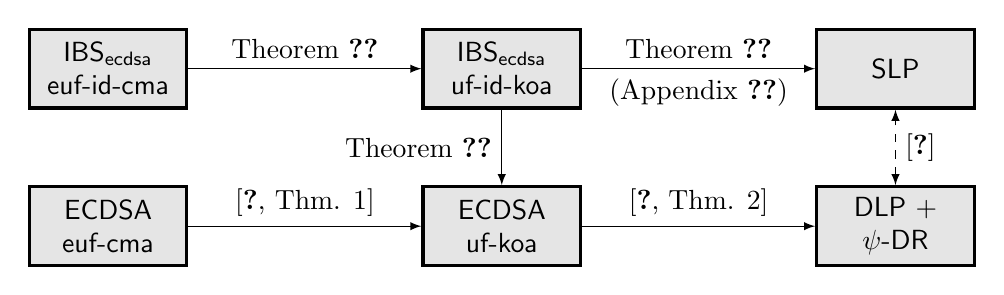
\begin{tikzpicture}[auto, node distance=5cm]
        \node[block] (eufcma) at (0,0) {\textsf{ECDSA}\\ \textsf{euf-cma}};
        \node[block, right of = eufcma] (ufkoa) {\textsf{ECDSA}\\ \textsf{uf-koa}};
        \node[block, right of = ufkoa] (dlp) {\textsf{DLP} +\\ $\psi$-\textsf{DR}};
        \node[block, above of = eufcma, node distance=2cm] (eufidcma) {$\mathsf{IBS}_{\mathsf{ecdsa}}$\\ \textsf{euf-id-cma}};
        \node[block, right of = eufidcma] (ufidkoa) {$\mathsf{IBS}_{\mathsf{ecdsa}}$\\ \textsf{uf-id-koa}};
        \node[block, right of = ufidkoa] (slp) {\textsf{SLP}};
        \draw[-latex] (eufcma) -- node[above] {\cite[Thm. 1]{CCS:FerKilPoe16}} (ufkoa);
        \draw[-latex] (ufkoa) -- node[above] {\cite[Thm. 2]{CCS:FerKilPoe16}} (dlp);
        \draw[-latex] (eufidcma) -- node[above] {Theorem \ref{thm:euf}} (ufidkoa);
        \draw[-latex] (ufidkoa) -- node[left] {Theorem \ref{thm: ufidkoa to ufkoa}} (ufkoa);
        \draw[-latex] (ufidkoa.east) -- node[above] {Theorem \ref{thm:ko}} node[below] {(Appendix \ref{appendix: ufidkoa to slp})} (slp.west);
        \draw[latex-latex, dashed] (dlp.north) -- node[right] {\cite{Fersch2017}} (slp.south);
        % \draw[-latex, dashed] (ufidkoa.south east) -- (dlp.north west);
    \end{tikzpicture}
    \caption{Summary of the security proof under \textsc{GenDSA}'s framework. The dashed line represents an equivalent result.}
    \label{fig: contributions}
\end{figure}

\item \emph{Comparison between our scheme and Galindo-Garcia's}: we evaluate the performance between our ECDSA-based scheme and Schnorr-like scheme with hierarchical delegation of public key, and discuss the usage of our scheme in scenarios with native ECDSA support in delegated credentials, e.g., OAuth2 and JSON Web Tokens.
\end{enumerate}

\noindent\textbf{Paper Outline.} The rest of the paper is organized as follows. 
%
Section \ref{sec:preliminaries} defines the notation, the model in which we will study our scheme, and the cryptographic assumptions used through the security analysis.
%
Section \ref{sec: galindo and garcia} discusses the core ideas of the Galindo-Garcia identity-based signature scheme, emphasizing their challenges and obtained results.
%
Section \ref{sec:ecdsa-ibs} defines the proposed scheme.
%
Section \ref{sec:security-proof} details the proof itself using a game-based strategy.
%
Section \ref{sec:results} analyzes the obtained performance of our scheme when compared to Galindo-Garcia's and presents applications that could benefit from our scheme. 
%
Section \ref{sec:conclusion} concludes the work.

\section{Preliminaries}\label{sec:preliminaries}

\subsection{Notation}
\noindent\underline{\textsc{Sets}.} For any finite set $S$, $x \sample S$ denotes the uniformly random sampling of an element $x \in S$ and $|S|$ is the number of elements. 
% 
We use the notation $\Interval{n}$ to write the numbers from $1$ to $n$ and $\Interval{m:n}$ to represent the numbers from $m$ to $n \ge m$. 
% 
Finally, $\left\{0,1\right\}^{\ast}$ is the set of all binary strings with arbitrary finite size.

\noindent\underline{\textsc{Algebra}.} Through the paper we write $\Zp := \mathbb{Z}/p\mathbb{Z}$ as the ring of integers modulo prime number $p$, and $\Zpplus := \Zp\backslash\{0\}$. For an Abelian group $\Group$ written additively with neutral element $\mathcal{O}$ (in the case of elliptic curves, this is the point at infinity), we write $\Group^{*} := \Group / \{\mathcal{O}\}$. For elliptic curves, let $q$ be a prime number, $E/\Group$ be an elliptic curve, $\EllipticCurve$ the set of points with coordinates defined over $\Fq\times\Fq$ such that $|\EllipticCurve| = p$ indicates the number of elements of this set and $pG = \mathcal{O}$ where $G$ is called the generator of the curve. 
%

\noindent\underline{\textsc{Security Games}.} We call $\mathcal{A}$ an attacker on our scheme and write $\mathcal{A}^{\mathsf{O}_{1}, \mathsf{O}_{2},\ldots,\mathsf{O}_{n}}$ when the attacker has access to oracles $\mathsf{O}_{i \in \Interval{n}}$, while $\mathcal{C}$ represents the challenger. We use $\mathcal{AMS}$ letters $\mathcal{A}$, $\mathcal{B}$, and $\mathcal{F}$ to represent attackers. We use $x \leftarrow \mathsf{A}$ to say that $x$ is the output of a deterministic algorithm $\mathsf{A}$ while $x \xleftarrow{\$} \mathsf{A}$ when the algorithm is probabilistic. The security parameter is represented by $\ lambda$. The string $1^{\lambda}$ consists of only $1$ as a digit and has a length of $\lambda$. During the proof, we use code-based security games \cite{RogwayEprint2004, Rogway2006}. A game $\mathbf{G}$ is defined as a probability experiment in which an adversary $\Attacker$ interacts with an implicit challenger $\Challenger$ that answers oracle queries posed by $\Attacker$. More formally, a game is a sequence of programs such that $\mathbf{G} = \left(\mathsf{Init}, \mathsf{P_{1}}, \ldots, \mathsf{P_{n}}, \mathsf{Finalize}\right)$ where $\mathsf{P}_{i \in \Interval{n}}$ are the \emph{oracles} of the game. The binary output $b$ of the $i$--th game $\mathbf{G}_{i}$ between the challenger $\Challenger$ and the attacker $\Attacker$ is denoted by $\mathbf{G}_{i}^{\Attacker} \Rightarrow b$. The attacker \emph{wins} if $b = 1$. Lastly, we use colored boxes to indicate changes between consecutive games and highlight their differences.

\noindent\underline{\textsc{Oracles and Hash Functions}.} We use \textsf{sans serif fonts} to represent an oracle illustrating some idealized cryptographic primitive, e.g., $\mathsf{O}$. 
%
We represent $\#\mathsf{O}\left(x\right)$ as the index on which the oracle query to input $x$ was made, $\left|\mathsf{O}\right|$ as the range of elements in $\mathsf{O}$'s table and $q_{\mathsf{O}}$ as the maximum number of queries allowed. 
%
The attacker can make as many queries $x_{i}$ to $\mathsf{O}\left(.\right)$ as he/she wants and obtain $\mathsf{O}\left(x_{i}\right)$ as output. 
%
The table associated with the oracle is represented by $\mathfrak{L}$. The entries of this table are defined according to the oracle's arguments. 
%
Finally, when dealing with tables, the associated query is represented by enclosed brackets, e.g., $\Braket{a_{i}, b_{i},\ldots, z_{i}}$ where $a,b,\ldots, z$ are the entries of the table. 
%
Digests of hash functions are presented by $h$ (or  $h', h''$, etc, when this is the case).

\noindent\underline{\textsc{Color Schema}.} Finally, we use different colors to represent pairs of keys, signatures, points on the curve, and others for conciseness. Public keys (or points on the curve) are represented with upper case letters in
\textcolor{blue}{blue}, generators are represented in \textcolor{BurntOrange}{orange}, and private keys are represented in \textcolor{red}{red}. Signatures are written in \textcolor{Sepia}{brown}. Forgeries are written in \textcolor{magenta}{magenta} and a star $^{\star}$ (for example $\textcolor{magenta}{\sigma^{\star}}$ represents a forjed signature). Nonces are represented in \textcolor{Green}{green}, digests are written in \textcolor{cyan}{cyan}, and commitments in \textcolor{Plum}{purple}.\label{sec:color-schema}
\subsection{Modeling the Conversion Function of ECDSA}\label{subsec:conversion-function}

The conversion function is given by $f: \EllipticCurve \mapsto \Zp$, mapping a point $Q \in \EllipticCurve$ to its $x$--coordinate modulo prime number $p$, i.e., $f\left(Q\right) = x \bmod{p},\ Q := \left(x, y\right) \in \Fq\times\Fq$ without preserving a visible algebraic structure, meaning that the only connection between its domain and its range seems to be that $|\Group| = |\Zp|$. However, practical instantiations of $f$ are not bijective, thus resulting that $|\ProjFunction{\Group}| < |\Zp|$ as highlighted by \cite{CCS:FerKilPoe16}. Guided by those pieces of evidence, the most recent analysis of ECDSA relies on modeling $f$ by combining its disruptive algebraic nature and real-world properties. Fersch et al. model $f$ as a composition of functions, i.e., $f(x) = \left(\psi \circ \Pi \circ \varphi\right)(x)$. 

We use the following notation to represent the (co)domain of functions $\psi, \Pi, \varphi$: $\mathbb{A}$ contains binary strings $\alpha \in \{0,1\}^{\lambda},\ \lambda := \lceil\log_{2}{q}\rceil$ with $2^{\lambda} \le q < 2^{\lambda+1}$; $\mathbb{B}$ corresponds to the interval $\Interval{2^{\lambda}-1}$. Every element of $\mathbb{B}$ is represented by $\beta$. Both $\psi$ and $\varphi$ are fast and efficient functions. Function $\varphi$ reflects the structure of $f$ that involves only its domain, i.e., it maps a point on the curve onto its representation as a binary string of length $\lambda$:\[
    \varphi: \EllipticCurve \mapsto \mathbb{A} \subseteq \{0,1\}^{\lambda}
\]

Function $\psi$ reflects the structure of $f$'s range by mapping a point onto its $x$-coordinate modulo $p$. The novelty of this model is to use $\Pi$ as a bijection to disrupt any algebraic link between the domain and the range of $f$. In our case, $\varphi$ is such that any two elliptic curve points $P$ and $P'$ with the same $x$--component will be mapped to the same element, and function $\psi$ is the \emph{modulo $p$ function} that implements the characteristic bias of the range of $f$. Note that $f$ is invertible since both $\varphi$ and $\psi$ are invertible. More formally, $\varphi$ is a semi-injective function (or 2-to-1).

\begin{definition}[\textbf{Semi-Injective Function}, \cite{Kiltz2023}]\label{definition: semi-injective function}
Let $\Group$ be a prime order group and $\mathbb{D}$ a set. A function $\varphi:\Group^{*} \rightarrow \mathbb{D}$ is called semi-injective if\begin{enumerate}[label={\emph{\roman*})}]
\item its range $\varphi\left(\Group^{*}\right) \subseteq \mathbb{D}$ is efficiently decidable and
\item it is either injective or a 2-to-1 function, i.e.,  $\varphi\left(x\right) = \varphi\left(y\right) \Longrightarrow x \in \left\{y, y^{-1}\right\}$.
\end{enumerate}
\end{definition}

\begin{corollary}[\cite{Kiltz2023}]\label{corollary: psi quantity}
Let $\psi : \mathbb{B} \mapsto \Zp$  be a semi-injective function to which we associate the quantity:
\[
    \varepsilon_{\psi} = \underset{t \in \Zp}{\max} \underset{{0 \le y < 2^{\lambda}}}{\mathrm{Pr}}  \left(\psi(y) = t\right)
\]    
Then, the value of $\varepsilon_\psi$ is bounded above by $2/p$.
\end{corollary}

\begin{definition}[\textbf{Bijective Random Oracle}]
A bijective random oracle, hereby represented by $\mathsf{bRO}$, is an idealized public bijection that is accessible, in both directions, via oracles. We model $\Pi$ as a $\mathsf{bRO}$ to write the security proof. We write $\DirectOracle$ and $\InverseOracle$ as oracles. $\DirectOracle$ is defined as follows:\[
\Pi: \{0,1\}^{\lambda} \mapsto \Interval{2^{\lambda}-1}
\]

Note that $\ProjFunction{\pm X_{i}} = x_{i}$ due to the symmetry of the elliptic curve with respect to the horizontal axis. As $\Pi$ corresponds to the bijective random oracle, as per usual, we use two lists, $\mathfrak{L}_{\DirectOracle}$ and $\mathfrak{L}_{\InverseOracle}$ to represent the pair of values $\left(\alpha, \beta\right) \in \mathbb{A} \times \mathbb{B}$ such that $\Pi \subseteq \mathbb{A} \times \mathbb{B}$. For a general element of $\Zp$, we use $t$ which is equals to $\psi\left(\beta\right)$ for some $\beta \in \mathbb{B}$. Finally, one can easily write the following relation for $P \in \EllipticCurve$ where $\alpha \in \mathbb{A}$ and $\beta \in \mathbb{B}$:\[
    \varphi\left(P\right) = \alpha,\ \Pi\left(\alpha\right) = \beta \iff \Pi^{-1}\left(\beta\right) = \alpha,\ \psi\left(\beta\right) = t \in \Zp
\]
\end{definition}

\subsection{Identity-Based Signature Schemes}

Identity-based signature schemes are a cryptographic primitive derived from the seminal work by Shamir \cite{Shamir1985}. He first introduced an identity-based setting where the necessity of exchanging private and public keys was removed due to the existence of a \emph{trusted} authority that issues the user's secret key using a master secret. The trusted authority is commonly referred to as the key generation center (KGC) or Trusted Third Party (TTP).

\begin{definition}[\textbf{Identity-based Signature}] 
An identity-based signature scheme $\mathsf{IBS}$ is a tuple of four efficient algorithms $\mathsf{IBS} = \left(\mathsf{Setup}, \mathsf{KeyDeriv}, \mathsf{Sign}, \mathsf{Verify}\right)$ defined as follows:\begin{enumerate}[label={\emph{\roman*})}]
    \item $\mathsf{Setup}(\lambda)$: the $\mathsf{Setup}$ algorithm is responsible for generating the master key pair $\left(\msk, \mpk\right)$ upon input the security parameter $\lambda$
    \item $\KeyDeriv{\msk, \id{}}$: based on the user's identifier $\id{}$, the trusted authority performs the key derivation algorithm to obtain the user's secret key, i.e., $\mathsf{sk}_{\id{}} \leftarrow \KeyDeriv{\msk, \id{}}$, and sends it back to the user
    \item $\Sign{\id{}, \msg{}, \sk{}_{\id{}}}$: the signing algorithms proceeds as usual producing a signature $\Signature{}$ on the digest of $\msg{}$ and $\id{}$ with the user's private signing key $\sk_{\id{}}$
    \item $\Verify{\Signature{}, \id{}, \msg{}, \mpk}$: the verification algorithm outputs the value $b = 1$ if the signature is valid over the message $\msg{}$ and the $\id{}$ using $\mpk$ as public verification key, and $b = 0$ otherwise.
\end{enumerate}
\end{definition}

The security model used to prove the security of the IBS is a variant of the known existential unforgeability under adaptive chosen-message attack \cite{Goldwasser1984}, which is extended by appending the identity attack \cite{Gentry2002}.\begin{definition}[\textbf{EUF--ID--CMA Game}]\label{def: euf-id-cma}
    An adversary $\adv$ is said to break the existential unforgeability under chosen-message and identity attack game against the identity-based signature scheme $\mathsf{IBS}$ if, after receiving the master public key, he can produce a forged signature on a new identity and a new identity-message pair that has never been queried. The adversary is given access to two oracles, the extraction and signing oracles ($\ExtractionOracle$ and $\SignatureOracle$, respectively). The first, upon receiving a query on the $\id{}$, returns the user's private key $\sk_{\id{}}$, while the second produces a signature after being queried on a pair $(\msg{}, \id{})$. The advantage of $\adv$ winning the game is given by
    \begin{equation}
    \mathsf{Adv}_{\adv, \mathsf{IBS}}^{\mathsf{euf}\text{-}\mathsf{id}\text{-}\mathsf{cma}}(\lambda) =
    \Probability{\begin{array}{ll}
        \\
        1 \leftarrow \Verify{\Forge{\sigma}, \Forge{\id{}}, \Forge{\msg{}}} \\
        \\ 
    \end{array} \left|
    \begin{array}{ll}
        \left(\Forge{\sigma}, \Forge{\id{}}, \Forge{\msg{}}\right) \leftarrow \adv^{\ExtractionOracle,\SignatureOracle}(\mpk), \\
        \Braket{\Forge{\id{}}} \notin\mathfrak{L}_{\mathsf{ext}},\ \Braket{\Forge{\id{}}, \Forge{\msg{}}} \notin \mathfrak{L}_{\mathsf{sig}},\\ 
        (\mpk, \msk) \sample \mathsf{SetUp}(\lambda)  \\
    \end{array}\right.
    }
    \end{equation}
\end{definition}

A weaker, but still useful security notion, is the \emph{unforgeability under key-only attacks}. In this setting, the games proceed as a usual chosen-message attack game with one difference: the attacker is not allowed to pose signing queries to the signing oracle. We define this notion in the identity-based setting as follows:
\begin{definition}[\textbf{UF-ID-KOA Game}]\label{def: uf-id-koa}
    An adversary $\adv$ is said to break the unforgeability under key-only and identity attack game against the identity-based signature scheme $\mathsf{IBS}$ if, after receiving the master public key, he can produce a forged signature on a new identity and a new identity-message pair that has never been queried. The adversary is given access to the extraction oracle only, which performs as Definition \ref{def: euf-id-cma}. The advantage of $\adv$ winning the game is given by
    \begin{equation}
        \mathsf{Adv}_{\adv, \mathsf{IBS}}^{\mathsf{uf}\text{-}\mathsf{id}\text{-}\mathsf{koa}}(\lambda) =
    \Probability{\begin{array}{ll}
        \\
        1 \leftarrow \Verify{\Forge{\sigma}, \Forge{\id{}}, \Forge{\msg{}}} \\
        \\ 
    \end{array} 
    \left|
    \begin{array}{ll}
        \left(\Forge{\sigma}, \Forge{\id{}}, \Forge{\msg{}}\right) \leftarrow \adv^{\ExtractionOracle}(\mpk),\\
        \Braket{\Forge{\id{}}} \notin \mathfrak{L}_{\mathsf{ext}},\\
        (\mpk, \msk) \sample \mathsf{SetUp}(\lambda)  \\
    \end{array}\right.
    % }
    }
    \end{equation}
\end{definition}

\subsection{Cryptographic Assumptions}

\begin{definition}[\textbf{Discrete Logarithm Problem}]\label{def: dlp}
Let $\left(\Group, G, p\right)$ be a prime-order group. An adversary $\Attacker$ is said to $\left(t_{\mathsf{dl}}, \varepsilon_{\mathsf{dl}}\right)$--break the discrete logarithm problem if, upon receiving $X := xG$ from challenger $\mathcal{C}$, it runs in time $t \le t_{\mathsf{dl}}$ and has an advantage
\begin{equation}\label{eq:dlp}
    \mathsf{Adv}_{\Attacker, \Challenger}^{\mathsf{dlp}}(\lambda) := 
    \Probability{
    \begin{array}{ll}
    \\
    \Hat{x} = x\ \\
    \\
    \end{array}
    \left|
    \begin{array}{ll}
    \Hat{x} \leftarrow \Attacker\left(X\right),\\
    x \sample\Zpplus,\ X = xG,\\
    (\Group, G, p) \leftarrow \mathsf{G}(\lambda)
    \end{array}
    \right.} = \varepsilon_{\mathsf{dl}}
\end{equation}
\end{definition}

\begin{definition}[\textbf{Semi-Logarithm Problem}, \cite{Fersch2017}]\label{def: slp}
Let $\left(\Group, G, p\right)$ be a prime-order group, $f$ a function mapping elements from $\Group^{\ast}$ to $\Zp$, and $\rho_{0},\rho_{1}: \Zp^{2}\mapsto \Zp$ functions. An adversary $\Attacker$ is said to $\left(t_{\mathsf{slp}}, \varepsilon_{\mathsf{slp}}\right)$--break the semi-logarithm problem in $\Group$ with respect to $f, \rho_{0}, \rho_{1}$ if, upon receiving $X := xG$ from challenger $\Challenger$, it runs in time $t \le t_{\mathsf{slp}}$ and has an advantage
\begin{equation}\label{eq:slp}
    \mathsf{Adv}_{\Attacker, \Challenger}^{\mathsf{slpp}}(\lambda) := 
    \Probability{
    \begin{array}{ll}
    \\
    v = \ProjFunction{\rho_{0}(u, v)G + \rho_{1}(u,v)X} \\
    \\
    \end{array}
    \left|
    \begin{array}{ll}
    \left(u, v\right) \leftarrow \Attacker\left(X\right),\\
    x \sample\Zpplus,\ X = xG,\\
    (\Group, G, p) \leftarrow \mathsf{G}(\lambda)
    \end{array}
    \right.} = \varepsilon_{\mathsf{slp}}
\end{equation}
\end{definition}
For both Definitions \ref{def: dlp} and \ref{def: slp}, we consider that group $\Group$ is represented by the elliptic curve $\EllipticCurve$ such that its order is equal to $p$.

\begin{definition}[\textbf{Collision Resistance of a Hash Function}]
Let $\HashFunctionH: \{0,1\}^{\ast} \mapsto \Zp$ be a hash function. An adversary $\Attacker$ is said to $\left(t_{\mathsf{cr}, \HashFunctionH}, \varepsilon_{\mathsf{cr}, \HashFunctionH}\right)$--break the collision resistance of hash function $\HashFunctionH$ if it finds two distinct messages with equal digests in time $t \le t_{\mathsf{cr}, \HashFunctionH}$ and with advantage \begin{equation}\label{eq:collision-resistance}
    \mathsf{Adv}_{\Attacker, \HashFunctionH}^{\mathsf{cr}}(\lambda) = 
    \Probability{\begin{array}{ll}
    \\
    \HashH{\msg{1}} = \HashH{\msg{0}}\\
    \\
    \end{array}
    \left|
    \begin{array}{ll}
    \msg{0} \neq \msg{1},\\
    \msg{0}, \msg{1} \in \{0,1\}^{\ast},\\
    (\msg{0}, \msg{1}) \leftarrow \adv(\cdot)
    \end{array}\right.} = \varepsilon_{\mathsf{cr}, \HashFunctionH}
\end{equation}
\end{definition}

\begin{definition}[$\psi$\textbf{--Relative Division Resistance of a Hash Function}, \cite{CCS:FerKilPoe16}]
Let $\HashFunctionH: \{0,1\}^{\ast} \mapsto \Zp$ be a hash function, $\mathbb{B}$ a set, and $\psi: \mathbb{B} \mapsto \Zp$ a function. Let $\mathbb{B}^{\ast} = \psi^{-1}\left(\Zpplus\right)$. We say an adversary $\Attacker = \left(\adv_{1}, \adv_{2}\right)$ $\left(t_{\mathsf{dr}, \HashFunctionH}, \varepsilon_{\mathsf{dr}, \HashFunctionH}\right)$--breaks the $\psi$--relative division resistance of $\HashFunctionH$ if it runs in time $t \le t_{\mathsf{dr}, \HashFunctionH}$ and has an advantage \begin{equation}\label{eq:psi-resistance-division-resistance}
    \mathsf{Adv}_{\Attacker, \HashFunctionH}^{\mathsf{dr}}(\lambda) = 
    \Probability{
    \begin{array}{ll}
    \\
    \dfrac{\HashH{\msg{1}}}{\psi\left(\beta_{1}\right)} = \dfrac{\HashH{\msg{0}}}{\psi\left(\beta_{0}\right)} \\
    \\
    \end{array}
    \left|
    \begin{array}{ll}
    \beta_{0}, \beta_{1} \sample \mathbb{B}^{\ast},\\
    \left(\msg{0}, \Gamma\right) \sample \adv_{1}\left(\beta_{0}\right),\\
    \msg{1} \sample \adv_{2}\left(\Gamma, \beta_{1}\right)
    \end{array}\right.
    } = \varepsilon_{\mathsf{dr}, \HashFunctionH}
\end{equation}
Here, $\Gamma$ is some arbitrary state information passed from $\adv_{1}$ to $\adv_{2}$.
\end{definition}

\begin{lemma}[\cite{CCS:FerKilPoe16}]
    If an attacker can find messages $\msg{}$ and $\msg{}'$ (not necessarily distinct) such that, for two values, $\beta$ and $\beta'$, the relation $\dfrac{\HashH{\msg{}}}{\psi\left(\beta\right)} = \dfrac{\HashH{\Forge{\msg{}}}}{\psi\left(\Forge{\beta}\right)}$ is obtained, then he/she can produce a forgery on signature $\Forge{\sigma} = \left(\Forge{u}, \Forge{t}\right)$ over message $\Forge{\msg{}}$. Hence, the adversary is said to \emph{break the $\psi$--division resistance of hash function $\HashFunctionH$}.
\end{lemma}
\begin{proof}
    Let $\Signature{} = \left(s, t\right),\ s = \Nonce{r^{-1}}\left(\HashH{\msg{}} + t\PrivKey{z}\right),\ t = \ProjFunction{\Commitment{R}} = \psi\left(\beta\right)$. We show that the attacker can produce a forgery $\Forge{\sigma} = \left(\Forge{s}, \Forge{t}\right)$ over message $\Forge{\msg{}}$, as follows\[
        s\Nonce{r} = \HashH{\msg{}} + t\PrivKey{z} \Rightarrow s\dfrac{\Nonce{r}}{t} = \dfrac{\Digest{h}}{t} + \PrivKey{z} = \dfrac{\Forge{h}}{\Forge{t}} + \PrivKey{z} \therefore s\Nonce{r}\dfrac{\Forge{t}}{t} = \Forge{h} + \Forge{t}\PrivKey{z}  \xRightarrow{\times G} s\dfrac{\Forge{h}}{\Digest{h}}\Commitment{R} = \Forge{h}\GeneratorEC + \Forge{t}\PubKey{Z}
    \]
    Thus, $\Forge{s} = s\Forge{h}/\Digest{h}$ and $\Forge{\sigma} = \left(s\Forge{h}/\Digest{h}, \Forge{t}\right)$.
\end{proof}

In terms of analysis of the Schnorr signature scheme, the General Forking Lemma is a historically used mathematical tool. The proof consists on finding collisions in $\Commitment{R}$ by manipulating the random oracle to respond queries with values $\Commitment{R} := s\GeneratorEC - \Digest{h}\PubKey{Z},\ \Digest{h} := \HashH{\Commitment{R}, \msg{}}$, and extract the signing key $\PrivKey{z}$, thus proving a relation between the advantage of forging a signature and solving the discrete logarithm problem. The idea is shown as follows: if the adversary can produce a forgery by rewinding the random oracle $\Forge{\sigma} = (\Forge{R}, \Forge{s}),\ \Commitment{R} = \Forge{R}$, on the forged message $\Forge{\msg{}}$, then he can extract the discrete logarithm $\PrivKey{z} := \log_{\GeneratorEC}^{\Group}\PubKey{Z}$:
\begin{equation}\label{eq: schnorr-extraction}
         \Commitment{R} = \Forge{R} \Rightarrow s\GeneratorEC - \Digest{h}\PubKey{Z} = \Forge{s}\GeneratorEC - \Forge{h}\PubKey{Z} \therefore \PrivKey{z} = \dfrac{\Forge{s} - s}{\Forge{h} - \Digest{h}} \bmod{p}
\end{equation}

ECDSA has a similar reasoning. Now the attacker tries to find collisions between the values of the conversion function: assume that two signatures $\Signature{} = \left(u, t\right)$ and $ \Forge{\sigma} = \left(\Forge{u}, \Forge{t}\right)$ are obtained, respectively, on messages $\msg{}$ and $\Forge{\msg{}}$, the idea is to find $R,\ \Forge{R}$ such that $R = \eta \Forge{R},\ |\eta| = 1$. This means obtaining the following relation:
\begin{equation}\label{eq:ecdsa-extraction}
    t\PubKey{Z} = \Forge{t}\PubKey{Z} \Rightarrow \left(\eta s - \Forge{s}\right)\Forge{R} = \left(\Digest{h} - \Forge{h}\right)\GeneratorEC \therefore  \PrivKey{z} = \dfrac{\Forge{s}\Digest{h} - \eta s\Forge{h}}{\Forge{t}\left(\eta s - \Forge{s}\right)}\bmod{p}
\end{equation}

Where $\Digest{h} := \HashH{\msg{}},\ \Forge{h} := \HashH{\Forge{\msg{}}}$. By modeling the projection function $f$ as a bijective random oracle, we implicitly allow the usage of Theorem \ref{thm:general-forking-lemma} to rewind the oracle until conveniently finding a collision (i.e., $R=\eta\Forge{R}$) and extracting the discrete logarithm.



\section{Galindo-Garcia IBS}\label{sec: galindo and garcia}

The work by Galindo and Garcia proposed a construction of IBS using two concatenated Schnorr signatures, leveraging the simplicity and the efficiency of such signatures \cite{Galindo2009}. While the technique itself is not new, it has been widely studied when applied to different scenarios. Examples range from identity-based encryption schemes to public key infrastructure-related primitives. The scheme is shown in Definition \ref{def:galindo-garcia} by considering a group $\Group$ of prime order $p$ written multiplicatively and generated by $\GeneratorSchnorr$.
\begin{definition}[\textbf{Galindo-Garcia IBS}]\label{def:galindo-garcia}
  The scheme is represented by the tuple of four efficient algorithms $\mathsf{IBS}_{\mathsf{Sch.GG}} := \left(\mathsf{SetUp},\ \mathsf{KeyDeriv},\ \mathsf{Sign},\ \mathsf{Verify}\right)$ and follows the sequence of steps described below:
  \begin{enumerate}[label={\emph{\roman*}})]
    \item $\mathsf{SetUp}\left(\lambda\right)$: upon receiving the security parameter and having public access to the DLP instance $\Delta = \left(g, p, \Group\right)$, the algorithm first generates $\PrivKey{z} \sample \Zp$ and define $\PubKey{Z} := \GeneratorSchnorr^{\PrivKey{z}}$. Set $\msk = \PrivKey{z}$ and $\mpk = \left(\Group, p, \GeneratorSchnorr, \PubKey{Z}, \mathsf{H}, \mathsf{G}\right)$ where $\mathsf{H}$ and $\mathsf{G}$ are hash functions mapping from $\left\{0,1\right\}^{*}$ to $\Zp$. It finally returns $\left(\mpk, \msk\right)$

    \item $\mathsf{KeyDeriv}\left(\msk, \id{}\right)$: using the master public key and the user's identifier, the trusted authority samples $\Nonce{r} \sample \Zp$, sets $\Commitment{R} := \GeneratorSchnorr^{\Nonce{r}}$ and obtains the digest $\Digest{h} := \mathsf{H}\left(\Commitment{R},\id{}\right)$. Finally, it defines the user's secret key $\PrivKey{\sk_{\id{}}} := \left(y, \Commitment{R}\right)$ where $y := \Nonce{r} + \PrivKey{z}\Digest{h}\bmod{p}$;

    \item $\mathsf{Sign}\left(\id, \msg{}, \PrivKey{\sk_{\id{}}}\right)$: on inputs $\PrivKey{\sk_{\id{}}} = \left(y, \Commitment{R}\right)$ and $\id{}$, the user signs the hash of the message $\msg{}$ by setting $\Commitment{A} := \GeneratorSchnorr^{\Nonce{a}}$ where $\Nonce{a} \sample \Zp$, and obtaining the signature $\Signature{} = \left(\Commitment{A}, b, \Commitment{R}\right) \in \Group \times \Zp \times \Group$ where $b := \Nonce{a} + y\Digest{h'} \bmod{p},\ \Digest{h'} := \mathsf{G}\left(\id{}, \Commitment{A}, \msg{}\right)$;

    \item $\mathsf{Verify}\left(\Signature{}, \id{}, \msg{}, \mpk\right)$: the verification algorithm is done by first calculating both digests, i.e., $\Digest{h} = \HashH{\Commitment{R}, \id{}}$ and $\Digest{h'} = \HashG{\id{}, \Commitment{A}, \msg{}}$ and then evaluating if the following equality holds:\[ 
      \GeneratorSchnorr^{b} \overset{?}{=} \Commitment{A}\left(\Commitment{R}\PubKey{Z}^{\Digest{h}}\right)^{\Digest{h'}}
      \] 
  \end{enumerate}
\end{definition}

This scheme is proven secure under the EUF-ID-CMA game by constructing two reductions that solve the discrete logarithm problem using the rewinding technique related to the General Forking Lemma (Theorem \ref{thm:general-forking-lemma}) \cite{CCS:BelNev06} and to the Multiple Forking Lemma (Theorem \ref{thm:multiple-forking-lemma}) \cite{Boldyreva2012}. It is worth mentioning that the work by Chatterjee et al. highlights some of the problems in the formal analysis and proposes a correct security proof. We refer to the author's original work for a more detailed discussion \cite{Chatterjee2012}. All in all, the Galindo-Garcia IBS offers a smaller number of exponentiations and shorter signatures compared to \cite{Herranz2006, Barreto2005}, relatively recent work at the time, and represents an attractive option in resource-constrained scenarios.

\begin{theorem}[\textbf{General Forking Lemma}]\label{thm:general-forking-lemma}
    Fix $q \in \mathbb{Z}^{+}$ and a set $\mathbb{S}$ such that $|\mathbb{S}| \ge 2$. Let $\mathcal{W}$ be a randomized algorithm that on input string $x$ and elements $s_{1},\ldots,s_{q} \in \mathbb{S}$ returns a pair $\left(I,\sigma\right)$ consisting of an integer $0 \le I \le q$ and a string $\sigma$. The forking algorithm $\mathcal{F}_{\mathcal{W}}$ associated to $\mathcal{W}$. The algorithm $\mathcal{F}_{\mathcal{W}}\left(x\right)$ returns $\left(1,\sigma_{0},\sigma_{1}\right)$ in case of success and $\left(0,\bot,\bot\right)$ in case of failure. Let $\mathsf{G}_{1}$ be a randomized algorithm that takes no input and returns a string. Let\[
        \mathsf{acc} := \prob{x\sample \mathsf{G}_{1}; s_{1}^{0},\ldots,s_{\gamma}^{0} \sample \mathbb{S};\ \left(I_{0},\sigma_{0}\right) \sample \mathcal{W}\left(x, s_{1}^{0},\ldots,s_{\gamma}^{0}\right) | I_{0} \ge 1}
    \]
    And\[
        \mathsf{gfrk} := \prob{x \sample \mathsf{G}_{1}; \left(b, \sigma_{0}, \sigma_{1}\right) \sample \mathcal{F}_{\mathcal{W}}(x)| b = 1}
    \]
    Then\[
        \mathsf{gfrk} \ge \mathsf{acc}\left(\dfrac{\mathsf{acc}}{\gamma} - \dfrac{1}{|\mathbb{S}|}\right)
    \]
\end{theorem}

\begin{theorem}[\textbf{Multiple Forking Lemma}]\label{thm:multiple-forking-lemma}
        Fix a positive integer $q$ and a set $\mathbb{S}$ with at least two elements. Let $n$ be and odd integer and $\mathcal{M}_{\mathcal{W},n}\left(x\right)$ be the multiple forking algorithm over $\mathcal{W}$ that returns the tuple $\left(I, J, \sigma\right)$ with $0 \le J < I \le q,\ q \in \mathbb{Z}_{>0}$. On the other hand, $\mathcal{M}$ returns $\left(1, \left\{\sigma_{0},\ldots, \sigma_{n}\right\}\right)$ in case of success and $\left(0, \bot\right)$. Let $\mathsf{G}_{1}$ be a randomized algorithm that takes no input and returns a string, and $\mathsf{acc}$ is defined as follows:\[
            \mathsf{acc} := \prob{x\sample \mathsf{G}_{1}; s_{1}^{0},\ldots,s_{\gamma}^{0} \sample \mathbb{S};\ \left(I_{0},\sigma_{0}\right) \sample \mathcal{W}\left(x, s_{1}^{0},\ldots,s_{\gamma}^{0}\right) | I_{0} \ge 1 \cap J_{0} \ge 1}
        \]
        And\[
            \mathsf{mfrk} := \prob{x \sample \mathsf{G}_{1}; \left(b, \mathsf{results}\right) \sample \mathcal{M}_{\mathcal{W}, n}(x)| b = 1}
        \]
        Then\[
            \mathsf{mfrk} \ge \mathsf{acc}\left(\dfrac{\mathsf{acc}^{n}}{\gamma^{2n}} - \dfrac{n}{|\mathbb{S}|}\right)
        \]
\end{theorem}
    
\section{Proposed Scheme}\label{sec:ecdsa-ibs}
\begin{definition}\label{def:ecdsa-ibs}
    Our identity-based signature scheme $\mathsf{IBS}_{\mathsf{ecdsa}}  \left(\mathsf{Setup}, \mathsf{KeyDeriv}, \mathsf{Sign}, \mathsf{Verify}\right)$ is a tuple of four efficient algorithms defined as follows:
    \begin{enumerate}[label={\emph{\roman*})}]
        \item $\Setup{\lambda}$: upon input $\lambda$ and public access to a DLP--instance $\Delta := \left(\EllipticCurve, q, \GeneratorEC, p\right)$, it generates the master key pair $\left(\msk, \mpk\right) := \left(\PrivKey{z}, \PubKey{Z} := \PrivKey{z}\GeneratorEC\right)$ such that $\PrivKey{z} \sample \Zpplus$

        \item $\KeyDeriv{\msk, \id{}}$: the trusted authority generates a random nonce $\Nonce{r}$, sets $\Commitment{R} := \Nonce{r}\GeneratorEC$, calculates $t := \ProjFunction{\Commitment{R}}$, $\Digest{h} := \HashH{\id{}}$, and $u := \Nonce{r^{-1}}\left(\Digest{h} +t\PrivKey{z}\right)\bmod{p}$. $\PrivKey{\sk_{\id{}}} = \left(u, t\right)$ is returned;
        
        \item $\Sign{\PrivKey{\sk_{\id{}}}, \msg{}, \id{}}$: the user takes $\PrivKey{u}$ as private signing key, $\Generator{R} := \PrivKey{u}^{-1}\left(\Digest{h}\GeneratorEC + t\PubKey{Z}\right)$  (correctness of the first signature) as generator, and the verification key $\PubKey{U} := \PrivKey{u}\Generator{R}$. The rest of the algorithm proceeds as usual.

        \item $\Verify{\Signature{}, \msg{}, \mpk, \id{}}$: $\Signature{}$ is parsed into $\left(u', t', \Generator{R}\right)$ to obtain $t = \ProjFunction{\Generator{R}},\ \Digest{h} := \HashH{\id{}}$, and $\Digest{h'} := \HashG{\msg{}, \id{}}$. Using $\PubKey{Z} := \mpk$,
        it recovers $\Commitment{R'} = u'^{-1}\left(\Digest{h'}\Commitment{R} + t'\Digest{h}\GeneratorEC + t't\PubKey{Z}\right)$ and outputs the boolean value of $t' \overset{?}{=} \ProjFunction{\Commitment{R'}}$.
    \end{enumerate}
\end{definition}

Part of the importance of this work lies in some aspects when considering the usage of ECDSA-like schemes and identity-based signature schemes with hierarchical delegation of public keys. 
%
Usual ECDSA performs, during verification phase, the following steps considering a signature $\Signature{} = \left(s, t\right)$ on message $\msg{}$: (\textit{i}) $\Digest{h} := \HashH{\msg{}}$, (\textit{ii}) $\Commitment{R} := s^{-1}\left(\Digest{h}\GeneratorEC + t\PubKey{Z}\right)$ with $\PubKey{Z}$ being the public verification key, and (\textit{iii}) outputs the boolean value of $\ProjFunction{\Commitment{R}} \overset{?}{=} t$. 
%

When considering real-world implementations, for example, information used as input of a hash function generally corresponds to messages, public keys, and commitments to avoid related-key attacks \cite{Bellare2003, Morita2015}. 
%
However, when embedding the commitment into the hash function, considering, for instance, a construction analog to Schnorr, the verification process becomes impossible since $\Commitment{R}$ is recovered based on $\Digest{h}$, in this case, equals to $\HashH{\Commitment{R}, \msg{}}$. 

A solution to this problem would be to consider using the public key $\PubKey{Z}$ of the signer alongside the message to be signed $\msg{}$ instead.
%
In such a case, the digest can be calculated so that the $\Commitment{R}$ is recovered.
%
The signing algorithm could be written as Figure \ref{fig: complete description-modified}. We denote this first variant of our scheme as $\mathsf{IBS}_{\mathsf{ecdsa}}^{\mathsf{v_{1}}}$.
%
Obtaining an ECDSA signature during the key extraction and signing phase is impossible to achieve simultaneously since verification requires more information to be carried out than what is contained in the signature. 
% 
In this case, the signing algorithm would proceed as in the right column of Figure \ref{fig: complete description-modified}. 
% 
However, by applying this reasoning to the signing algorithm, verification would depend on additional information to be carried, and consequently, more complex calculations would be required.
%
\begin{figure}[H]
    \centering
    \begin{pchstack}[center, boxed, space = 1em]
    \begin{pcvstack}
    \pseudocode[linenumbering, head = {$\mathsf{SetUp}(\lambda)$}]{
    \PrivKey{z} \sample \Zpplus\\
    \msk := \PrivKey{z} \\
    \PubKey{Z} := \PrivKey{z}\GeneratorEC\\
    \mpk := \PubKey{Z} \\
    \pcreturn \left(\mpk, \msk\right)
    }
    \pseudocode[linenumbering, head = {$\KeyDeriv{\msk, \id{}}$}]{
    \PrivKey{z} := \msk\\
    \Nonce{r} \sample \Zp\\
    \Commitment{R} := \Nonce{r}\GeneratorEC\\
    \pcif \Commitment{R} = \PointAtInfinity:\ \pcabort\\
    t = \ProjFunction{\Commitment{R}}\\
    \pcif t = 0:\ \pcabort\\
    \Digest{h} := \HashH{\id{}}\\
    u := \Nonce{r^{-1}}(\Digest{h} + t\PrivKey{z})\bmod{p}\\
    \pcreturn \PrivKey{\sk_{\id{}}} = (u, t)
    }
    \end{pcvstack}
    \begin{pcvstack}
    \pseudocode[linenumbering, head = {$\Sign{\PrivKey{\sk_{\id{}}}, \msg{}, \id{}}$}]{
    (\PrivKey{u}, t) := \PrivKey{\sk_{\id{}}}\\
    \PubKey{Z} := \mpk\\
    \Digest{h} := \HashH{\id{}}\\
    \Generator{R} := \PrivKey{u^{-1}}(\Digest{h}\GeneratorEC + t\PubKey{Z})\\
    \PubKey{U} := \PrivKey{u}\Generator{R}\label{sign:line2}\\
    \Nonce{r'} \sample \Zp\\
    \Commitment{R'} := \Nonce{r'}\Generator{R}\\
    \pcif \Commitment{R'} = \PointAtInfinity:\ \pcabort\\
    t' = \ProjFunction{\Commitment{R'}}\\
    \pcif t' = 0:\ \pcabort\\
    \Digest{h'} := \HashG{\msg{}, \id{}}\\
    s' := \Nonce{r'^{-1}}(\Digest{h'} + t'\PrivKey{u})\bmod{n}\\
    \pcreturn \Signature{} = (s', t', \Commitment{R})
    }
    \pseudocode[linenumbering, head = {$\Verify{\Signature{}, \msg{}, \mpk, \id{}}$}]{
    (s', t', \Generator{R}) := \Signature{}\\
    \pcif t' = 0 \cup s' = 0: \pcabort\\
    \PubKey{Z} := \mpk\\
    \Digest{h} := \HashH{\id{}}\\
    \Digest{h'} := \HashG{\msg{}, \id{}}\\
    t := \ProjFunction{\Generator{R}}\\
    \Commitment{R'} := s'^{-1}(\Digest{h'}\Generator{R} + t'(\Digest{h}\GeneratorEC + t\PubKey{Z})):\\
    \pcif t' \neq \ProjFunction{\Commitment{R'}}:\\
    \t \pcreturn \mathsf{false}\\
    \pcreturn \mathsf{true}
    }
    \end{pcvstack}
    \end{pchstack}
    \caption{Complete description of $\mathsf{IBS}_{\mathsf{ecdsa}}$. 
    }
    \label{fig: complete description}
\end{figure}


Also, in terms of security analysis, it would be required to find some other mathematical result instead of the Forking Lemma \cite{Pointcheval2000} when dealing with $\HashFunctionH$ since the fact of using $\mpk$ as an argument would not allow rewinding. Even though one single modification in the key derivation algorithm could be used to obtain an actual ECDSA signature as a private signing key, the implied consequences would still be an object of future study. Another possible implementation would be to use signatures as $\Signature{} = \left(u, \Commitment{R}\right)$ with $\ProjFunction{R} = t$, thus, \emph{implicitly}, obtaining a conventional ECDSA signature. 
%
By using this format while keeping commitment $\Commitment{R}$ as input of the hash function $\HashFunctionH$, we would obtain the verification equation as follows: $\left(u, \Commitment{R}\right) := \Signature{},\ \Digest{h} := \HashH{\Commitment{R}, \id{}},\ t:= \ProjFunction{\Commitment{R}},\ u\Commitment{R} \overset{?}{=} \Digest{h}\GeneratorEC + t\PubKey{X}$. This version we denote by $\mathsf{IBS}_{\mathsf{ecdsa}}^{\mathsf{v_{2}}}$ which is a Schnorr-like signature as the one proposed by Galindo and Garcia.
%
Using $u$ as private key, one can define $\PubKey{U} = \PrivKey{u}\Generator{R}$, samples $\Nonce{r'} \sample \Zp$, sets $\Commitment{R'} = \Nonce{r'}\Generator{R}$, obtain $t' = \ProjFunction{\Commitment{R'}}$ and $\Digest{h'} = \HashG{\PubKey{U},\msg{},\id{}}$, finally setting $u' = \Nonce{r'^{-1}}\left(\Digest{h'} + t'\PrivKey{u}\right)\bmod{n}$. The signature produced would be $\Signature{} = \left(u', \Commitment{R'}, \Generator{R}\right)$. Verification holds if $u'\Commitment{R'} \overset{?}{=} \Digest{h'}\Commitment{R} + t'\PubKey{U}$ for $U \overset{?}{=} \Digest{h}\GeneratorEC + t\PubKey{X},\ t = \ProjFunction{R}$. Note that the produced signature can still be of the form $\Signature{} = \left(u', t', \Generator{R}\right)$, an even closer variant of ECDSA. In such case, verification would consists of extracting $\Commitment{R'}$ by means of $\Commitment{R'} = u'^{-1}\left(\Digest{h'}\Generator{R} + t'\PubKey{U}\right)$ and comparing $t' \overset{?}{=} \ProjFunction{\Commitment{R'}}$. This variant would not work if $\Digest{h'} = \HashG{\Commitment{R'}, \msg{}, \id{}}$ since a circularity would be involved and, thus, only $\Signature{} = \left(u', \Commitment{R'}, \Generator{R}\right)$ would allow a possible variant.

Finally, a last discussed variant (hereby denoted by $\mathsf{IBS}_{\mathsf{ecdsa}}^{\mathsf{v_{3}}})$ would consist in the following modifications to the proposed scheme: (\emph{i}) during the $\mathsf{KeyDeriv}$ algorithm the obtained private key would be of the form $\PrivKey{\sk_{\id{}}} := \left(u, t, \Commitment{R}\right)$ where $t = \ProjFunction{\Commitment{R}}$, a ECDSA-like signature over $\Digest{h} := \HashH{\Commitment{R}, \id{}}$ and; (\emph{ii}) the produced signature $\Signature{}$ over $\Digest{h'}:= \HashG{\Commitment{R'}, \msg{}, \id{}}$ would be of the form $\left(u', \Commitment{R'}, \Generator{R}\right),\ \Commitment{R'} := \Nonce{r'}\Generator{R},\ \Nonce{r'} \sample \Zp$ thus; (\emph{iii}) verification would require solely the evaluation of $u'\Commitment{R'} \overset{?}{=} \Digest{h'}\Generator{R} + t'\Digest{h}\GeneratorEC + t't\PubKey{Z}$. This method, although allowing the least amount of operations and, especially, no inversion over $\Zp$, requires an even more convoluted security proof.

\begin{figure}[H]
    \centering
    \begin{pchstack}[center, boxed, space=1em]
    \pseudocode[linenumbering, head = {$\mathsf{IBS}_{\mathsf{ecdsa}}^{\mathsf{v_{1}}}.\KeyDeriv{\msk, \id{}}$}]{
    \PrivKey{z} := \msk\\
    \PubKey{Z} := \PrivKey{z}\GeneratorEC\\
    \Nonce{r} \sample \Zp\\
    \Commitment{R} := \Nonce{r}\GeneratorEC\\
    \pcif \Commitment{R} = \PointAtInfinity:\ \pcabort\\
    t = \ProjFunction{\Commitment{R}}\\
    \pcif t = 0:\ \pcabort\\
    \Digest{h} := \HashH{\PubKey{Z}, \id{}}\\
    u := \Nonce{r^{-1}}(\Digest{h} + t\PrivKey{z})\bmod{n}\\
    \pcreturn \PrivKey{\sk_{\id{}}} = (u, t, \Commitment{R})
    }
    \pseudocode[linenumbering, head = {$\mathsf{IBS}_{\mathsf{ecdsa}}^{\mathsf{v_{1}}}.\Sign{\sk_{\id{}}, \msg{}, \id{}}$}]{
    (u, t, \Commitment{R}) := \PrivKey{\sk_{\id{}}}\\
    % \Commitment{R} := u^{-1}(\Digest{h}\GeneratorEC + t\PubKey{Z})\\
    \PubKey{U} := \PrivKey{u}\Generator{R}\\
    \Nonce{r'} \sample \Zp\\
    \Commitment{R'} := \Nonce{r'}\Generator{R}\\
    \pcif \Commitment{R'} = \PointAtInfinity:\ \pcabort\\
    t' = \ProjFunction{\Commitment{R'}}\\
    \pcif t' = 0:\ \pcabort\\
    \Digest{h'} := \HashG{\PubKey{U}, \msg{}, \id{}}\\
    u' := \Nonce{r'^{-1}}(\Digest{h'} + t'\PrivKey{u})\bmod{n}\\
    \pcreturn \Signature{} = (u', t', \Commitment{R})
    }
    \end{pchstack}
    \caption{The modified key derivation algorithm produces the signer's private key as an ECDSA-like signature using the public keys as inputs of the hash functions.}
    \label{fig: complete description-modified}
\end{figure}

\section{Security Proof}\label{sec:security-proof}

In this section, we show the security proof of our scheme $\mathsf{IBS}_{\mathsf{ecdsa}}$ by proving two theorems. The first shows how unforgeability under key-only attack in the identity-based setting implies existential unforgeability under chosen-message and identity attacks, and the second shows how the hardness of the semi-logarithm problem implies unforgeability under key-only and identity attacks.

\begin{theorem}\label{thm:euf}
    Under the bijective random oracle model, if exists a p.p.t. adversary $\Forger$ that $\left(t, \varepsilon, \ExtractionQueries, \SignatureQueries, \QueriesBRO \right)$--breaks existential unforgeability of $\mathsf{IBS}_{\mathsf{ecdsa}}$, then exists a p.p.t. adversary $\Forger_{0}$ that $\left(t', \varepsilon'\right)$--breaks existential unforgeability of $\mathsf{IBS}_{\mathsf{ecdsa}}$ under key-only and identity attack and adversaries, $\Attacker_{1}$ and $\Attacker_{2}$, that $\left(t_{\mathsf{cr}, \HashFunctionH}, \varepsilon_{\mathsf{cr}, \HashFunctionH}\right)$ and $\left(t_{\mathsf{cr}, \HashFunctionG}, \varepsilon_{\mathsf{cr}, \HashFunctionG}\right)$--break collision resistance of $\HashFunctionH$ and $\HashFunctionG$, respectively, where
    \begin{equation}\label{eq: thm1}
         \varepsilon \le \varepsilon' + \varepsilon_{\mathsf{cr}, \HashFunctionH} + \varepsilon_{\mathsf{cr}, \HashFunctionG} + \dfrac{\left(q_{\Pi} + \mathcal{Q}\right)\left(\ExtractionQueries + 2\SignatureQueries\right)}{\left(p-1\right)/2 - \mathcal{Q}} 
    \end{equation}
    With $t' \ge t + \mathcal{O}\left(\SignatureQueries + \ExtractionQueries\right),\ t_{\mathsf{cr}} := t_{\mathsf{cr}, \HashFunctionH} + t_{\mathsf{cr}, \HashFunctionG} \ge t + \mathcal{O}\left(\ExtractionQueries + \SignatureQueries\right)$, and $\mathcal{Q} = \ExtractionQueries + \SignatureQueries + q_{\Pi}$, $\ExtractionQueries$.
\end{theorem}

\begin{proof}
    \underline{\textbf{Game} $\mathbf{G_{0}^{\Forger}}$}. This is the usual EUF-ID-CMA game, hence: $\Probability{\mathbf{G}_{0}^{\Forger} \Rightarrow 1} = \mathsf{Adv}_{\Forger, \mathsf{IBS}_{\mathsf{ecdsa}}}^{\mathsf{euf}\text{--}\mathsf{id}\text{--}\mathsf{cma}}\left(\lambda\right) \therefore \Probability{\mathbf{G}_{0}^{\Forger} \Rightarrow 1} = \varepsilon$.
    
    \begin{figure}[H]
        \centering
        \begin{pchstack}[center, boxed, space=1em]
                \begin{pcvstack}
                \pseudocode[linenumbering, head = {$\mathsf{Init}(\lambda)$}]{
                \Pi: \mathbb{A} \rightarrow \mathbb{B}\\
                \PrivKey{z} \sample \Znplus\\
                \PubKey{Z} := \PrivKey{z} \GeneratorEC\\
                \mpk := \PubKey{Z}\\
                \pcreturn \mpk
                }
                \pseudocode[linenumbering, head = {$\mathsf{bRO}(\alpha)$}]{
                \pcreturn \Pi(\alpha)
                }
                \pseudocode[linenumbering, head = {$\mathsf{bRO}^{-1}(\beta)$}]{
                \pcreturn \Pi^{-1}(\beta)
                }
                \pseudocode[linenumbering, head = {$\ExtractionOracle(\id{i})$}]{
                \pcif \Braket{\id{i}} \in \mathfrak{L}_{\mathsf{ext}}:\\
                \t \PrivKey{\sk{}_{\id{i}}} := (u_{i}, t_{i})\\
                \t \pcreturn \PrivKey{\sk{}_{\id{i}}}\\
                \Nonce{r_{i}} \sample \Zn\\
                \Commitment{R_{i}} := \Nonce{r_{i}} \GeneratorEC\\
                \pcif \Commitment{R_{i}} = \PointAtInfinity:\\
                \t \pcabort\\
                \alpha_{i} \leftarrow \varphi(\Commitment{R_{i}})\\
                \beta_{i} \leftarrow \Pi(\alpha_{i})\\
                t_{i} \leftarrow \psi(\beta_{i})\\
                \pcif t_{i} = 0:\\
                \t \pcabort\\
                \Digest{h_{i}} := \HashH{\id{i}}\\
                s_{i} := \Digest{h_{i}} + t_{i}\PrivKey{z}\\
                \pcif s_{i} = 0:\\
                \t \pcabort\\
                u_{i} = s_{i}/\Nonce{r_{i}}\\
                \PrivKey{\sk{}_{\id{i}}} = (u_{i}, t_{i})\\
                \pcreturn \PrivKey{\sk{}_{\id{i}}}
                }
            \end{pcvstack}
            \begin{pchstack}
                \pseudocode[linenumbering, head = {$\SignatureOracle(\id{j}, \msg{j})$}]{
                \pcif \Braket{\msg{j}, \id{j}} \in \mathfrak{L}_{\mathsf{sig}}:\\
                \t \Signature{j} := \SignatureOracle(\msg{j}, \id{j})\\
                \t \pcreturn \Signature{j}\\
                \PrivKey{\sk{}_{\id{j}}} := \ExtractionOracle(\id{j})\\
                (u_{j}, t_{j}) := \PrivKey{\sk{}_{\id{j}}}\\
                \Digest{h_{j}} := \HashH{\id{j}}\\
                \PubKey{Z} := \mpk\\
                \Commitment{R_{j}} := u_{j}^{-1}(\Digest{h_{j}}\GeneratorEC + t_{j}\PubKey{Z})\\
                \PubKey{U_{j}} := \PrivKey{u_{j}}\Generator{R_{j}}\\
                \Nonce{r_{j}'} \sample \Zn\\
                \Commitment{R_{j}'} := \Nonce{r_{j}'} \Generator{R_{j}}\\
                \pcif \Commitment{R_{j}'} = \PointAtInfinity:\\
                \t \pcabort\\
                \alpha_{j}' := \varphi(\Commitment{R_{j}'})\\
                \beta_{j}' := \Pi(\alpha_{j}')\\
                t_{j}' := \psi(\beta_{j}')\\
                \pcif t_{j}' = 0:\\
                \t \pcabort\\
                \Digest{h_{j}'} := \HashG{\msg{j}, \id{j}}\\
                s_{j}' := \Digest{h_{j}'} + t_{j}'\PrivKey{u_{j}}\\
                \pcif s_{j}' = 0:\\
                \t \pcabort\\
                u_{j}' := s_{j}'/\Nonce{r_{j}'}\\
                \Signature{j} := (u_{j}', t_{j}', \Generator{R_{j}})\\
                \pcreturn \Signature{j}
                }
                \pseudocode[linenumbering, head={$\Finalize{\sigma^{\star}, \msg{}^{\star}, \id{}^{\star}, \mpk}$}]{
                \gamechange{\pcfor $\Braket{\msg{}, \id{}} \in \mathfrak{L}_{\mathsf{sig}}$}\\
                \gamechange{\t\pcif $\HashG{\msg{}^{\star}, \id{}^{\star}} = \HashG{\msg{}, \id{}}$}:\\
                \gamechange{\t\t\pcabort}\\
                \gamechange{\pcendfor}\\
                \gamechange{\pcfor $\Braket{\id{}} \in \mathfrak{L}_{\mathsf{ext}}$}\\
                \gamechange{\t\pcif $\HashH{\id{}^{\star}} = \HashH{\id{}}$:}\\
                \gamechange{\t\t\pcabort}\\
                \gamechange{\pcendfor}\\
                \pcif \id{}^{\star} \in \mathfrak{L}_{\mathsf{ext}}:\\
                \t \pcabort\\
                \pcif \Braket{\id{}^{\star}, \msg{}^{\star}} \in \mathfrak{L}_{\mathsf{sig}}:\\
                \t \pcabort\\
                \PubKey{Z} := \mpk\\
                (u', t', \Generator{R}) := \sigma^{\star}\\
                \alpha := \varphi(\Generator{R})\\
                \beta := \Pi(\alpha)\\
                t := \psi(\beta)\\
                \Digest{h} := \HashH{\id{}^{\star}}\\
                \PubKey{U} := \Digest{h}\GeneratorEC + t\PubKey{Z}\\
                \pcif \PubKey{U} = \PointAtInfinity\\
                \t \pcabort\\
                \Digest{h'} := \HashG{\msg{}^{\star}, \id{}^{\star}}\\
                \Commitment{R'} \overset{?}{=} u'^{-1}(\Digest{h'}\Generator{R} + t'\PubKey{U})\\
                \alpha' := \varphi(\Commitment{R'})\\
                \beta' := \Pi(\alpha')\\
                \pcreturn t' \overset{?}{=} \psi(\beta')
                }
            \end{pchstack}
            \end{pchstack}
        \caption{Specification of the oracles used for games $\mathbf{G_{0}^{\Forger}}$ and $\mathbf{G_{1}^{\Forger}}$.}
        \label{fig:game0-and-game1}
    \end{figure}
    
    \noindent\underline{\textbf{Game} $\mathbf{G_{1}^{\Forger}}$}. Here, we consider the probability of finding a hash collision during the $\mathsf{Finalize}$ procedure. Neither hash functions are modeled as a random oracle, thus avoiding the usual strategies for modeling repeated (or brand new) queries. The time required is given by $t_{\mathsf{cr}} := t_{\mathsf{cr}, \HashFunctionH} + t_{\mathsf{cr}, \HashFunctionG} \ge t + \mathcal{O}\left(\ExtractionQueries + \SignatureQueries\right)$.    
    \begin{equation*}\label{eq:game1}
            \Probability{\mathbf{G}_{0}^{\Forger} \Rightarrow 1} = \Probability{\mathbf{G}_{1}^{\Forger} \Rightarrow 1 \cup \mathsf{collision}^{\HashFunctionH} \cup \mathsf{collision}^{\HashFunctionG}} \le \Probability{\mathbf{G}_{1}^{\Forger} \Rightarrow 1} + \varepsilon_{\mathsf{cr}, \HashFunctionH} + \varepsilon_{\mathsf{cr}, \HashFunctionG}
    \end{equation*}
    Figure \ref{fig:game0-and-game1} describes the procedures and oracles implementations for both Games $\mathbf{G}_{0}^{\Forger}$ and $\mathbf{G}_{1}^{\Forger}$.

    \noindent\underline{\textbf{Game} $\mathbf{G_{2}^{\Forger}}$}. In this Game, we introduce abort conditions during queries being made to the bijective random oracle.
    % 
    Figure \ref{fig:euf-id-cma-phase-game2} show the description of Game $\mathbf{G_{2}^{\Forger}}$.
    % 
    We divide the analysis into three events described as follows:
    
    \noindent\underline{Event $\mathsf{S}_{1}$}. When $\Forger$ queries the \textsf{bRO} either directly or implicitly (by querying the extraction or signing oracle), $|\Pi^{O}|$ increases, thus $|\Pi^{S}|$ decreases since $\Pi := \Pi^{O} \cup\Pi^{S}$. Lines $4$ of $\mathsf{bRO}^{\pm1}$ are executed $q_{\Pi}$ in total. The number of queries to the signing oracle is bounded by $\SignatureQueries$, while the number of queries to the extraction oracle is at most $\ExtractionQueries$. This gives us the probability of occurrence of event $\mathsf{S}_{1}$ bounded by: 
    \begin{equation}\label{eq: event S1}
        \Probability{\mathsf{S}_{1}} \le \dfrac{q_{\Pi}\left(\ExtractionQueries + \SignatureQueries\right)}{2^{\lambda} - \mathcal{Q}}.
    \end{equation}
    With $\mathcal{Q} = \ExtractionQueries + q_{\Pi} + \SignatureQueries$ being the sum of explicit ($q^{\mathsf{expl}}$) and implicit ($q^{\mathsf{impl}}$) queries made to each oracle, i.e.,
    \begin{equation*}
        \mathcal{Q} \le \underbrace{\left(\ExtractionQueries^{\mathsf{expl}} + q_{\Pi}^{\mathsf{impl}}\right)}_{\text{extraction phase}} + \underbrace{\left(\SignatureQueries^{\mathsf{expl}} + \ExtractionQueries^{\mathsf{impl}} + q_{\Pi}^{\mathsf{impl}}\right)}_{\text{signing phase}} + q_{\Pi}^{\mathsf{expl}}.
    \end{equation*}
    
    \noindent\underline{Event $\mathsf{S}_{2}$}. For event $\mathsf{S}_{2}$ we have, in line $12$ of procedure $\ExtractionOracle\left(\id{}\right)$, a value bounded above by $\left(\ExtractionQueries + q_{\Pi}\right)\ExtractionQueries/2^{\lambda}$, and for line $9$, using the semi-injective characteristic of $\varphi$, bounded by $2\left(\ExtractionQueries + q_{\Pi}\right)\ExtractionQueries/\left(p-1\right)$. Hence, we can show that $2/\left(p-1\right) \ge 2^{-\lambda}$ and the total probability of event $\mathsf{S}_{2}$ is bounded above by\begin{equation}\label{eq: event S2}
        \Probability{\mathsf{S}_{2}} \le \dfrac{\ExtractionQueries\left(\ExtractionQueries + q_{\Pi}\right)}{2^{\lambda}} + \dfrac{\ExtractionQueries\left(\ExtractionQueries + q_{\Pi}\right)}{\dfrac{p-1}{2}} \le \dfrac{2\ExtractionQueries\left(\ExtractionQueries + q_{\Pi}\right)}{\dfrac{p-1}{2}}.
    \end{equation}
    \noindent\underline{Event $\mathsf{S}_{3}$}. Due to the symmetry between $\mathsf{S}_{2}$ and $\event{S}_{3}$, we have:
    \begin{equation}\label{eq: event S3}
        \Probability{\mathsf{S}_{3}} \le \dfrac{\SignatureQueries \mathcal{Q}}{\dfrac{p-1}{2}}.
    \end{equation}
    Combining Equation \ref{eq: event S1}, \ref{eq: event S2}, and \ref{eq: event S3}, using $q \le 2^{\lambda + 1} + 1$, and $\ExtractionQueries + q_{\Pi} \le \SignatureQueries$, we have:
    \begin{equation*}
        \Probability{\mathbf{G}_{1}^{\Forger} \Rightarrow 1} \le \Probability{\mathbf{G}_{2}^{\Forger} \Rightarrow 1} + \dfrac{\left(q_{\Pi} + \mathcal{Q}\right)\left(\ExtractionQueries + 2\SignatureQueries\right)}{\dfrac{p-1}{2} - \mathcal{Q}}.
    \end{equation*}
    \noindent\underline{\textbf{Game} $\mathbf{G_{3}^{\Forger}}$}: from the specifications of Game $3$ in Figure \ref{fig:euf-id-cma-phase-game3} and Game $2$ in Figure \ref{fig:euf-id-cma-phase-game2} the difference resides at the different moments in which the abort can happen.
    %
    In Game $2$, the $\alpha$ value if defined accordingly to $\varphi\left(\Commitment{R_{i}}\right)$ and then $\beta_{i}$ is sampled over $\mathbb{B}$. 
    %
    In Game $3$, the order of operations is inverted.
    %
    Since the values of $\alpha$ and $\beta$ are randomly chosen, both Games $2$ and $3$ are indistinguishable, allowing us to write:\begin{equation*}
    \Probability{\mathbf{G}_{3}^{\Forger} \Rightarrow 1} = \Probability{\mathbf{G}_{2}^{\Forger} \Rightarrow 1}
    \end{equation*}
    
    \begin{figure}[H]
        \centering
        \begin{pchstack}[center, boxed, space=1em]
    \begin{pcvstack}
    \pseudocode[linenumbering, head = {$\mathsf{Init}(\lambda)$}]{
    \gamechange{$(\Pi^{O}, \Pi^{S}) = (\varnothing, \varnothing)$}\\
    \PrivKey{z} \sample \Zpplus \\
    \PubKey{Z} := \PrivKey{z} \GeneratorEC \\
    \pcreturn \PubKey{Z}
    }
    \pseudocode[linenumbering, head = {$\mathsf{bRO}(\alpha)$}]{
    \gamechange{\pcif $(\alpha,\ \cdot\ ) \in \Pi$:}\\
    \t \pcreturn \Pi(\alpha)\\
    \gamechange{$\beta \sample \mathbb{B}\backslash\mathsf{Rng}(\Pi^{O})$}\\
    \gamechange{\pcif $(\ \cdot\ , \beta) \in \Pi^{S}$:}\\
    \gamechange{\t \pcabort}\\
    \gamechange{$\Pi^{O} \leftarrow \Pi^{O} \cup \{(\alpha, \beta)\}$}\\
    \gamechange{\pcreturn $\beta$}
    }
    \pseudocode[linenumbering, head = {$\mathsf{bRO}^{-1}(\beta)$}]{
    \gamechange{$\pcif (\ \cdot\ , \beta) \in \Pi$:}\\
    \t \pcreturn \Pi^{-1}(\beta)\\
    \gamechange{$\alpha \sample \mathbb{A}\backslash\mathsf{Dom}(\Pi^{O})$}\\
    \gamechange{\pcif $(\alpha,\ \cdot\ )\in \Pi^{S}$:}\\
    \gamechange{\t \pcabort}\\
    \gamechange{$\Pi^{O} \leftarrow \Pi^{O} \cup \{(\alpha, \beta)\}$}\\
    \gamechange{\pcreturn $\alpha$}
    }
    \end{pcvstack}
    \pseudocode[linenumbering, head = {$\ExtractionOracle(\id{i})$}]{
    \pcif \Braket{\id{i}} \in \mathfrak{L}_{\mathsf{ext}}:\\
    \t \PrivKey{\sk{}_{\id{i}}} := (u_{i}, t_{i})\\
    \t \pcreturn \PrivKey{\sk{}_{\id{i}}}\\
    \Nonce{r_{i}} \sample \Zp\\
    \Commitment{R_{i}} := \Nonce{r_{i}} \GeneratorEC\\
    \pcif \Commitment{R_{i}} = \PointAtInfinity:\\
    \t \pcabort\\
    \alpha_{i} \leftarrow \varphi(\Commitment{R_{i}})\\
    \gamechange{\textbf{if} $(\alpha_{i},\ \cdot\ ) \in \Pi$:}\\
    \gamechange{\t \pcabort}\\
    \gamechange{$\beta_{i} \sample \mathbb{B}$}\\
    \gamechange{\textbf{if} $(\ \cdot\ ,\beta_{i}) \in \Pi$:}\\
    \gamechange{\t \pcabort}\\
    \gamechange{$\Pi^{S} \leftarrow \Pi^{S}\cup\{(\alpha_{i}, \beta_{i})\}$}\\
    t_{i} \leftarrow \psi(\beta_{i})\\
    \pcif t_{i} = 0:\\
    \t \pcabort\\
    \Digest{h_{i}} := \HashH{\id{i}}\\
    s_{i} := \Digest{h_{i}} + t_{i}\PrivKey{z}\\
    \pcif s_{i} = 0:\\
    \t \pcabort\\
    u_{i} = s_{i}/\Nonce{r_{i}}\\
    \PrivKey{\sk{}_{\id{i}}} = (u_{i}, t_{i})\\
    \pcreturn \PrivKey{\sk{}_{\id{i}}}
    }
    \pseudocode[linenumbering, head = {$\SignatureOracle(\id{j}, \msg{j})$}]{
    \pcif \Braket{\msg{j}, \id{j}} \in \mathfrak{L}_{\mathsf{sig}}:\\
    \t \Signature{j} := \SignatureOracle(\msg{j}, \id{j})\\
    \t \pcreturn \sigma_{j}\\
    \PrivKey{\sk{}_{\id{j}}} := \ExtractionOracle(\id{j})\\ %\pccomment{Call to extraction oracle}\\
    (u_{j}, t_{j}) := \PrivKey{\sk{}_{\id{j}}}\\
    \Digest{h_{j}} := \HashH{\id{j}}\\
    \PubKey{Z} := \mpk\\
    \Commitment{R_{j}} := u_{j}^{-1}(\Digest{h_{j}}\GeneratorEC + t\PubKey{Z})\\
    \PubKey{U_{j}} := \PrivKey{u_{j}}\Generator{R_{j}}\\
    \Nonce{r_{j}'} \sample \Zp\\
    \Commitment{R_{j}'} := \Nonce{r_{j}'} \Generator{R_{j}}\\
    \pcif \Commitment{R_{j}'} = \PointAtInfinity:\\
    \t \pcabort\\
    \alpha_{j}' := \varphi(\Commitment{R_{j}'})\\
    \gamechange{\textbf{if} $(\alpha_{j}',\ \cdot\ ) \in \Pi$:}\\
    \gamechange{\t \pcabort}\\
    \gamechange{$\beta_{j}' \sample \mathbb{B}$}\\
    \gamechange{\textbf{if} $(\ \cdot\ ,\beta_{j}') \in \Pi$:}\\
    \gamechange{\t \pcabort}\\
    \gamechange{$\Pi^{S} \leftarrow \Pi^{S}\cup\{(\alpha_{j}', \beta_{j}')\}$}\\
    t_{j}' := \psi(\beta_{j}')\\
    \pcif t_{j}' = 0:\\
    \t \pcabort\\
    \Digest{h_{j}'} := \HashG{\msg{j}, \id{j}}\\
    s_{j}' := \Digest{h_{j}'} + t_{j}'\PrivKey{u_{j}}\\
    \pcif s_{j}' = 0:\\
    \t \pcabort\\
    u_{j}' := s_{j}'/\Nonce{r_{j}'}\\
    \Signature{j} := (u_{j}', t_{j}', \Generator{R_{j}})\\
    \pcreturn \Signature{j}
    }
    \end{pchstack}
        \caption{Specification of the oracles used during game $\mathbf{G}_{2}^{\Forger}$ with changes with respect to $\mathbf{G}_{1}^{\Forger}$ highlighted.}
        \label{fig:euf-id-cma-phase-game2}
    \end{figure}
   
   \noindent\underline{\textbf{Forger} $\Forger_{0}$}. Game $3$ relates to the case where $\Forger_{0}$ tries to break the key-only unforgeability of our scheme. The argument is analogue to the one in \cite{CCS:FerKilPoe16}: assume $\Forger$ produces a forgery $\Forge{\sigma} = \left(\Forge{u'}, \Forge{t'}, \Forge{R}\right)$, i.e.,  $\Forge{u'}\Forge{r'} = \Forge{h'} + \Forge{t'}\Forge{u}$, on $\Braket{\Forge{\id{}}, \Forge{\msg{}}}$, then we have two cases: $\left(\Forge{\alpha'}, \Forge{\beta'}\right) \in \Pi^{S}$ or $\left(\Forge{\alpha'}, \Forge{\beta'}\right) \in \Pi^{O}$. In the first case, the pair was defined in lines 22 or 25 of the extraction or signing oracle, respectively. Meaning, $\Forger_{0}$ knows a signature $\Signature{i} = \left(u'_{i}, t'_{i}, R_{i}\right)$ such that the conditions of Equation \ref{eq:ecdsa-extraction} occur, and $\Forger_{0}$ extracts the user's secret key, thus winning the game. The case when the forged pair $(\alpha, \beta) \in \Pi^{O}$ follows with little adaptation, since $\Pi^{O}$ contains the list of elements updated by querying the bijective random oracle. This means, $\Forger$ succeeded and so did $\Forger_{0}$, i.e., $\Probability{\mathbf{G}_{3}^{\Forger} \Rightarrow 1} = \Probability{\mathbf{G}_{0}^{\Forger_{0}} \Rightarrow 1} = \mathsf{Adv}_{\Forger_{0}, \mathsf{IBS}_{\mathsf{ecdsa}}}^{\mathsf{uf}\text{-}\mathsf{id}\text{-}\mathsf{koa}}(\lambda)$. By combining all previous results, we obtain the desired result. Note that, for EUF-CMA, taking $\ExtractionQueries = 0$ and $q_{\Pi}\le \mathcal{Q}/2,\ \mathcal{Q} \rightarrow q_{\Pi} + \SignatureQueries$ we obtain the result obtained by \cite{CCS:FerKilPoe16}.
    \begin{figure}[H]
        \centering
        \begin{pchstack}[center, boxed, space=1em]
                \pseudocode[linenumbering, head = {$\ExtractionOracle\left(\id{i}\right)$}]{
                \pcif \id{i} \in \mathfrak{L}_{\mathsf{ext}}:\\
                \t \PrivKey{\sk{}_{\id{i}}} := \left(u_{i}, t_{i}\right)\\
                \t \pcreturn \PrivKey{\sk{}_{\id{i}}}\\
                \Nonce{r_{i}} \sample \Zn\\
                \Commitment{R_{i}} := \Nonce{r_{i}} \GeneratorEC\\
                \pcif \Commitment{R_{i}} = \PointAtInfinity:\\
                \t \pcabort\\
                \gamechange{$\beta_{i} \sample \mathbb{B}$}\\
                \gamechange{\pcif $\left(\ \cdot\ ,\beta_{i}\right) \in \Pi$:}\\
                \gamechange{\t \pcabort}\\
                t_{i} \leftarrow \psi\left(\beta_{i}\right)\\
                \pcif t_{i} = 0:\\
                \t \pcabort\\
                \Digest{h_{i}} := \HashH{\id{i}}\\
                s_{i} := \Digest{h_{i}} + t_{i}\PrivKey{z}\\
                \pcif s_{i} = 0:\\
                \t \pcabort\\
                u_{i} = s_{i}/\Nonce{r_{i}}\\
                \gamechange{$\alpha_{i} \leftarrow \varphi\left(\Commitment{R_{i}}\right)$}\\
                \gamechange{\pcif $\left(\alpha_{i},\ \cdot\ \right) \in \Pi$:}\\
                \gamechange{\t \pcabort}\\
                \gamechange{$\Pi^{S} \leftarrow \Pi^{S}\cup\{\left(\alpha_{i}, \beta_{i}\right)\}$}\\
                \PrivKey{\sk{}_{\id{i}}} = \left(u_{i}, t_{i}\right)\\
                \pcreturn \PrivKey{\sk{}_{\id{i}}}
                }
                \pseudocode[linenumbering, head = {$\SignatureOracle\left(\msg{j}, \id{j}\right)$}]{
                \pcif \left(\id{j}, \msg{j}\right) \in \mathfrak{L}_{\mathsf{sig}}:\\
                \t \Signature{j} := \SignatureOracle\left(\msg{j}, \id{j}\right)\\
                \t \pcreturn \Signature{j}\\
                \PrivKey{\sk{}_{\id{j}}} := \ExtractionOracle\left(\id{j}\right)\\ %\pccomment{Call to extraction oracle}\\
                \left(\PrivKey{u_{j}}, t_{j}\right) := \PrivKey{\sk{}_{\id{j}}}\\
                \PubKey{U_{j}} := \PrivKey{u_{j}}\Generator{R_{j}}\\
                \gamechange{$\beta_{j}' \sample \mathbb{B}$}\\
                \gamechange{\pcif $\left(\ \cdot\ ,\beta_{j}'\right) \in \Pi$:}\\
                \gamechange{\t \pcabort}\\
                t_{j}' := \psi\left(\beta_{j}'\right)\\
                \pcif t_{j}' = 0:\\
                \t \pcabort\\
                \gamechange{$\Nonce{r_{j}'} \sample \Zn$}\\
                \gamechange{$\Commitment{R_{j}'} := \Nonce{r_{j}'} \Generator{R_{j}}$}\\
                \gamechange{\pcif $\Commitment{R_{j}'} = \PointAtInfinity$:}\\
                \gamechange{\t \pcabort}\\
                \Digest{h_{j}'} := \HashG{\msg{j}, \id{j}}\\
                s_{j}' := \Digest{h_{j}'} + t_{j}'\PrivKey{u_{j}}\\
                \pcif s_{j}' = 0:\\
                \t \pcabort\\
                u_{j}' := s_{j}'/\Nonce{r_{j}'}\\
                \gamechange{$\alpha_{j}' := \varphi\left(\Commitment{R_{j}'}\right)$}\\
                \gamechange{\pcif $\left(\alpha_{j}',\ \cdot\ \right) \in \Pi$:}\\
                \gamechange{\t \pcabort}\\
                \gamechange{$\Pi^{S} \leftarrow \Pi^{S}\cup\{\left(\alpha_{j}', \beta_{j}'\right)\}$}\\
                \Signature{j} := \left(u_{j}', t_{j}', \Generator{R_{j}}\right)\\
                \pcreturn \Signature{j}
                }
                
            % \end{pchstack}
            \end{pchstack}
        \caption{Specification of $\mathbf{G}_{3}^{\Forger}$ resulted from \colorbox{gray!20}{changes} with respect to game $\mathbf{G}_{2}^{\Forger}$.}
        \label{fig:euf-id-cma-phase-game3}
    \end{figure}
\end{proof}

\begin{theorem}\label{thm: ufidkoa to ufkoa}
    In the bijective random oracle model, if exists an p.p.t adversary $\Forger$ that $\left(t, \varepsilon, \ExtractionQueries, q_{\Pi}\right)$--breaks the unforgeability under identity and key-only attack of $\mathsf{IBS}_{\mathsf{ecdsa}}$, then exists a p.p.t. adversaries $\Forger_{0}$ that $\left(t', \varepsilon'\right)$--breaks the unforgeability under key-only attack of $\mathsf{ECDSA}$ and $\bdv$ that $\left(t_{\mathsf{cr,H}}, \varepsilon_{\mathsf{cr, H}}\right)$--breaks the collision resistance of hash function $\HashFunctionH$ where
    \[
        \varepsilon \le \left(\sqrt{2\QueriesBRO} + 1\right)\varepsilon' + \varepsilon_{\mathsf{cr}, \HashFunctionG},\ t' \ge t + \mathcal{O}\left(\sqrt{\QueriesBRO}\right)
    \]
\end{theorem}

\begin{proof}
    The game starts with $\Challenger$ generating a master key pair $\left(\msk, \mpk\right) \sample \mathsf{IBS}_{\mathsf{ecdsa}}.\mathsf{Init}\left(\lambda\right)$ accordingly to $\mathsf{IBS}_{\mathsf{ecdsa}}$'s description (Definition \ref{def:ecdsa-ibs}), and sending challenge $\mpk$ to forger $\Forger_{0}$. The forger is allowed only to pose queries to the \textsf{bRO}.
    %
    $\Forger_{0}$ then passes the $\mpk$ to forger $\Forger$.
    %
    $\Forger$ is allowed to query the extraction oracle $\ExtractionOracle$ on $\id{}$ and the \textsf{bRO}, and attempts to produce a valid forged signature on a brand new message-identity pair accordingly to Definition \ref{def: uf-id-koa}.
    %

    The idea of the proof is described as follows.
    %
    Every query posed by $\Forger$ to the extraction oracle is seen by $\Forger_{0}$, which in turn monitors the values queried in his/her table.
    %
    We denote this table by $\mathfrak{L}_{\mathsf{ext}, \Forger_{0}}$.
    %
    The same happens when oracle $\mathsf{bRO}^{\pm1}$ is queried.
    %
    $\Forger_{0}$ keeps track of queries with tables $\mathfrak{L}_{\DirectOracle, \Forger_{0}}$ and $\mathfrak{L}_{\InverseOracle, \Forger_{0}}$.
    %
    For each query that $\Forger$ poses to the extraction oracle, the oracle returns $\sk_{\id{}} := \ExtractionOracle\left(\id{}\right)$ as specified in Figure \ref{fig:game0-and-game1}.
    %
    $\Forger_{0}$ passes the challenge $\mpk$ to forger $\Forger$ as the second tries to break unforgeability under identity and key-only attack, i.e., produce a forged signature $\Forge{\sigma} = \left(\Forge{u'}, \Forge{t'}, \Forge{R}\right)$ on a brand-new identity-message pair.

    $\Forger_{0}$ wins when \emph{i}) $\Forger$ outputs a forgery $\Forge{\sigma_{0}} = \left(\Forge{u_{0}'}, \Forge{t_{0}'}, \Forge{R}\right)$, and \emph{ii}) rewinds $\Forger$ until it obtains another signature $\Forge{\sigma_{1}} = \left(\Forge{u_{1}'}, \Forge{t_{1}'}, \Forge{R}\right)$ on the same $u_{\id{}}$ such that $\Forge{t_{0}'} = \Forge{t_{1}'},\ \id{}^{\star} \notin \mathfrak{L}_{\mathsf{ext}}$.
    %
    Hence, using Equation \ref{eq:ecdsa-extraction} with $r_{1}' = \eta r_{0}'$, $\Forger_{0}$ calculates $r_{0}'$ and extracts $u_{\id{}^{\star}}$:\begin{equation}
        r_{0'} = \dfrac{h_{0}' - h_{1}'}{t_{0}'\left(u_{0}' - \eta u_{1}'\right)} \therefore u_{\id{}^{\star}} = \dfrac{u_{0}'h_{1}' - \eta u_{1}'h_{0}'}{t_{0}'\left(\eta u_{1}' - u_{0}'\right)}.
    \end{equation}
    Finally, $\Forger_{0}$ uses $\Forge{R}$ to calculate $\Forge{t} = \ProjFunction{\Forge{R}}$, and outputs $\left(u_{\id{}}, \Forge{t}\right)$, winning the UF-KOA game.
    %
    All in all, we can bound the probability of $\Forger_{0}$ being successful using the General Forking Lemma:\begin{equation*}
        \varepsilon' \ge \mathsf{acc}\left(\dfrac{\mathsf{acc}}{\QueriesBRO} - \dfrac{1}{2^{\lambda}}\right)
    \end{equation*}
    Where $\mathsf{acc} = \varepsilon - \varepsilon' - \varepsilon_{\mathsf{cr}, \HashFunctionG}$.
    %
    Manipulating the equation, we can consider two cases:
    \begin{case}
        If $\dfrac{\mathsf{acc}}{2\QueriesBRO} < \dfrac{1}{2^{\lambda}} \le \dfrac{\mathsf{acc}}{\QueriesBRO}$, then\begin{equation}
            \varepsilon \le \varepsilon' + \varepsilon_{\mathsf{cr}, \HashFunctionG} + \dfrac{2\QueriesBRO}{2^{\lambda}}
        \end{equation}
    \end{case}
    \begin{case}
        If $\dfrac{\mathsf{1}}{2^{\lambda}} \le \dfrac{\mathsf{acc}}{2\QueriesBRO}$, then\begin{equation}
            \varepsilon' \ge \dfrac{\mathsf{acc}^{2}}{2\QueriesBRO} \therefore \varepsilon \le \left(\sqrt{2\QueriesBRO} + 1\right)\varepsilon' + \varepsilon_{\mathsf{cr}, \HashFunctionG}
        \end{equation}
    \end{case}
\end{proof}

\section{Results}\label{sec:results}

In this section, we present the results obtained from algorithm analysis and by simulating identity-based ECDSA and Schnorr signature algorithms with hierarchical public key delegation. We start by analyzing the algorithms (Tables \ref{table: algorithmic comparison} and \ref{table: signature size}), evaluating the number of operations performed by each scheme.\\

\noindent\textbf{Algorithmic Analysis}. As presented in Section \ref{sec:ecdsa-ibs}, we propose different ECDSA-like identity-based schemes that support signature concatenation employing the Hierarchical Public Key Delegation technique. In Table \ref{table: algorithmic comparison}, these different schemes are compared in terms of algorithmic efficiency when considering the following operations: \emph{i}) sum, multiplication, and inversion over $\Zp$ are represented by $\mathsf{sum}$, $\mathsf{mul}$, and $\mathsf{inv}$, respectively, \emph{ii}) for \underline{p}oint \underline{ad}dition and \underline{m}ultiplication \underline{b}y \underline{s}calar we use $\mathsf{pad}$ and $\mathsf{mbs}$, and \emph{iii}) for hash operations, we use $\mathsf{hsh}$. As expected, our scheme has a higher algorithmic complexity since it lacks the linear property of Galindo-Garcia's scheme.

In terms of signature size $|\sigma|$, Table \ref{table: signature size} shows that the obtained ECDSA-like signatures are smaller than Galindo-Garcia IBS, $2|\Zpplus| + |\Group^{\ast}|$ instead of $|\Zpplus| + 2|\Group^{\ast}|$. This is a trade-off between $\mathsf{IBS}_{\mathsf{ecdsa}}$'s higher algorithmic complexity and smaller signatures due to ECDSA's non-linear structure and more convoluted verification steps regarding the recovery of commitment $R$ to further compare it to $\ProjFunction{R}$ during verification.
\begin{table}[H]
    \centering
    \begin{tabular}{c|r|r|r}
         \hline IBS & \multicolumn{1}{c|}{\textsf{KeyDeriv}} & \multicolumn{1}{c|}{\textsf{Sign}} & \multicolumn{1}{c}{\textsf{Verify}} \\
         \hline $\mathsf{IBS}_{\mathsf{GG}}$ & $\mathsf{mbs}, \mathsf{hsh}, \mathsf{sum}, \mathsf{mul}$ & $\mathsf{mbs}, \mathsf{hsh}, \mathsf{sum}, \mathsf{mul}$ & $2 \mathsf{pad}, 5\mathsf{mbs}, 2\mathsf{hsh}$ \\
         \hline $\mathsf{IBS}_{\mathsf{ecdsa}}$ & $\mathsf{mbs}, \mathsf{hsh}, \mathsf{sum}, \mathsf{inv}, 2\mathsf{mul}$ & $3\mathsf{mbs}, 2\mathsf{hsh}, 2\mathsf{sum}, 2\mathsf{inv}, 4\mathsf{mul}$ & $5\mathsf{pad}, 2\mathsf{mbs}, 2\mathsf{hsh}, \mathsf{inv}$ \\
         
         \hline $\mathsf{IBS}_{\mathsf{ecdsa}}^{\mathsf{v}_{1}}$ & \multicolumn{1}{c|}{-} & $3\mathsf{mbs}, 2\mathsf{hsh}, 2\mathsf{sum}, 2\mathsf{inv}, 4\mathsf{mul}$ & $5\mathsf{pad}, 2\mathsf{mbs}, 2\mathsf{hsh}, \mathsf{inv}$ \\
         
         \hline $\mathsf{IBS}_{\mathsf{ecdsa}}^{\mathsf{v}_{2}}$ & \multicolumn{1}{c|}{-} & $2\mathsf{mbs}, \mathsf{hsh}, \mathsf{sum}, \mathsf{inv}, \mathsf{mul}$ & $3\mathsf{pad}, 4\mathsf{mbs}, 2\mathsf{hsh}$ \\
         \hline $\mathsf{IBS}_{\mathsf{ecdsa}}^{\mathsf{v}_{3}}$ & \multicolumn{1}{c|}{-} & $2\mathsf{mbs}, \mathsf{hsh}, \mathsf{sum}, \mathsf{inv}, \mathsf{mul}$ & $3\mathsf{pad}, 4\mathsf{mbs}, 2\mathsf{hsh}$\\
         \hline
    \end{tabular}
    \caption{Algorithmic analysis of key-derivation, sign, and verify algorithms comparing the variants of identity-based ECDSA and \cite{Galindo2009} scheme.}
    \label{table: algorithmic comparison}
\end{table}


\begin{table}[H]
    \centering
    \begin{tabular}{c|c|c}
         \hline & $\sigma$ & $|\sigma|$\\
         \hline $\mathsf{IBS}_{\mathsf{GG}}$ & $\left(A, b, R\right)$ & $|\Zp| + 2|\Group^{\ast}|$ \\
         \hline $\mathsf{IBS}_{\mathsf{ecdsa}}$ & $\left(u', t', R\right)$ & $2|\Zp| + |\Group^{\ast}|$ \\
         \hline $\mathsf{IBS}_{\mathsf{ecdsa}}^{\mathsf{v}_{1}}$ & $\left(u', t', R\right)$ & $2|\Zp| + |\Group^{\ast}|$ \\
         \hline $\mathsf{IBS}_{\mathsf{ecdsa}}^{\mathsf{v}_{2}}$ & $\left(u', t', R\right)$ & $2|\Zp| + |\Group^{\ast}|$ \\
         \hline $\mathsf{IBS}_{\mathsf{ecdsa}}^{\mathsf{v}_{3}}$ & $\left(u', R', R\right)$ & $|\Zp| + 2|\Group^{\ast}|$ \\
         \hline
    \end{tabular}
    \caption{Comparison of signature's format and size between Galindo-Garcia's IBS and $\mathsf{IBS}_{\mathsf{ecdsa}}$.}
    \label{table: signature size}
\end{table}

\noindent\textbf{Baseline Results}. During the experiments, we use a highly optimized elliptic curve library implemented in C to compare our implementations using OpenSSL.
%
Table \ref{table: comparison openssl vs. bitcoin-core} aims to show these minor differences between ECDSA and Schnorr when considering a native implementation (OpenSSL implements ECDSA in its libraries, but does not implement Schnorr) versus a non-native implementation (Schnorr's signature algorithm with OpenSSL).
%
Our results represent the same tendency when comparing the algorithms in ECDSA and Schnorr.
%
While Schnorr is faster when signing, ECDSA's verification performs faster. Further, based on these codes, we compare the performance of Galindo-Garcia's IBS and ours using OpenSSL.
%
Our scheme performs slightly faster during key derivation and signing algorithms, as we can see in Table \ref{table: comparison ibsecdsa vs. ibsschnorr}.

\begin{table}[H]
\centering
\begin{tabular}{ccc|cc}
\cline{2-5}
\multicolumn{1}{l}{} & \multicolumn{2}{c|}{\textsf{ECDSA} avg. performance in $\si{\milli\second}$} & \multicolumn{2}{c}{\textsf{Schnorr} avg. performance in $\si{\milli\second}$} \\ \cline{2-5} 
\multicolumn{1}{l}{} & OpenSSL         & Baseline Result & OpenSSL         & Baseline Result \\ \hline
$\mathsf{KeyGen}$    & $2.40 \pm 0.38$ & $ 0.29 $ & $2.80 \pm 0.52$ & $ 0.29  $ \\ \hline
$\mathsf{Sign}$      & $0.89 \pm 0.18$ & $ 0.39 $ & $0.61 \pm 0.17$ & $ 0.27 $ \\ \hline
$\mathsf{Verify}$    & $0.55 \pm 0.12$ & $ 0.58 $ & $1.20 \pm 0.32$ & $ 0.62 $ \\ \hline
\end{tabular}
\caption{Comparison between \textsf{ECDSA} and \textsf{Schnorr} algorithm instantiated over \textsf{secp256k1} using OpenSSL (our implementation) and the baseline result using the \textsf{bitcoin-core} repository \cite{secp256k1} -- a highly optimized implementation of both algorithms over elliptic curve \textsf{secp256k1}.}
\label{table: comparison openssl vs. bitcoin-core}
\end{table}

\begin{table}[ht!]
\centering
\begin{tabular}{cc|c}
\cline{2-3}
\multicolumn{1}{l}{} & $\mathsf{IBS}_{\mathsf{ecdsa}}$ & $\mathsf{IBS}_{\mathsf{GG}}$ \\ \hline
$\mathsf{KeyDeriv}$  & $0.82 \pm 0.30$                 & $1.23 \pm 0.35$              \\ \hline
$\mathsf{Sign}$      & $0.66 \pm 0.24$                 & $0.69 \pm 0.18$              \\ \hline
\end{tabular}
\caption{Average performance comparison between the hierarchical delegation of public key technique applied to ECDSA and the Schnorr algorithm.}
\label{table: comparison ibsecdsa vs. ibsschnorr}
\end{table}


\section{Conclusion}\label{sec:conclusion}

In this paper, we present the first ECDSA-like identity-based signature scheme that allows signature concatenation, employing the Hierarchical Delegation of Public Key technique, which leverages the cyclic property of the group. 
%
Our security analysis combines the \emph{existential unforgeability under chosen-message and chosen identity attack game} -- EUF-ID-CMA game -- by embedding the modeling of the conversion function as a bijective random oracle.
%
We demonstrate that the security of our scheme can be reduced to ECDSA's unforgeability under key-only attacks in Section \ref{sec:security-proof} (a result by \cite{CCS:FerKilPoe16}). Additionally, we present an optional security proof in Appendix \ref{appendix: ufidkoa to slp}, which reduces the security of our scheme to the semi-logarithm problem.
%
We also show a reduction from our scheme to the discrete logarithm problem in two steps, following the strategy of Fersch et al.

In terms of performance, even with a more convoluted algorithmic structure during signing and verification, our scheme works slightly more efficiently than the Galindo-Garcia Schnorr-like identity-based scheme.
%
All in all, it represents an interesting application in cloud-oriented authentication systems due to its support for ECDSA, and opens up interesting possibilities in hierarchical delegation token scenarios and secure credential management.

\section*{Aknowledgments}
This study was financed in part by Hewlett Packard Enterprise (HPE), and by the following Brazilian research engines: FAPESP (grant 2020/09850-0), CNPq (grant 307732/2023-1), and Coordenação de Aperfeiçoamento de Pessoal de Nível Superior -- Brasil (CAPES) -- (Finance Code 001).

\bibliography{abbrev3, crypto, biblio}

\appendix
\section{From UF-ID-KOA to SLP}\label{appendix: ufidkoa to slp}
\begin{theorem}\label{thm:ko}
    Under the bijective random oracle model, if there exists a forger $\Forger_{0}$ that $\left(\varepsilon, t, \QueriesBRO \right)$--breaks unforgeability of $\mathsf{IBS}_{\mathsf{ecdsa}}$ under chosen identity and key-only attack, then there exists an algorithm $\Attacker$ that $\left(\varepsilon_{\mathsf{slp}}, t_{\mathsf{slp}}\right)$--breaks the semi-logarithm problem, where\[
         \varepsilon \le \varepsilon_{\mathsf{slp}} + \dfrac{\QueriesBRO^{2}}{2^{\lambda}} + \sqrt{2\QueriesBRO\varepsilon_{\mathsf{slp}}}
    \]
    With $t_{\mathsf{slp}} \ge t + \mathcal{O}\left(\QueriesBRO\right)$.
\end{theorem}

\begin{proof}
\noindent\underline{\textbf{Game} $\mathbf{G_{0}^{\Forger_{0}}}$}. The first game corresponds to the chosen identity and key-only attack by forger $\Forger_{0}$ when interacting with a challenger $\Challenger$. Upon receiving the challenge value $\PubKey{Z}$ corresponding to the \emph{master public key}, $\Forger_{0}$ tries to output a valid forgery. Finally, one can write:\[
    \Probability{\mathbf{G}_{0}^{\Forger_{0}} \Rightarrow 1} = \mathsf{Adv}_{\Forger_{0}, \mathsf{IBS}_{\mathsf{ecdsa}}}^{\mathsf{uf}\text{-}\mathsf{id}\text{-}\mathsf{koa}}\left(\lambda\right) \therefore \Probability{\mathbf{G}_{0}^{\Forger_{0}} \Rightarrow 1} = \varepsilon
\]

\noindent\underline{\textbf{Game} $\mathbf{G_{1}}$}. In this game, we introduce the abort condition during queries to the bijective random oracle and to the extraction oracle.
%
\begin{figure}[H]
\centering
\begin{pchstack}[center, boxed, space=1em]
\begin{pcvstack}
\pseudocode[linenumbering, head = {$\mathsf{Init}(\lambda)$}]{
(\Pi_{\rightarrow}, \Pi_{\leftarrow}) = (\varnothing, \varnothing)\\
\PrivKey{z} \sample \Zpplus \\
\msk := \PrivKey{z}\\
\PubKey{Z} := \PrivKey{z}\GeneratorEC \\
\mpk := \PubKey{Z}\\
\pcreturn \mpk
}
\pseudocode[linenumbering, head = {$\mathsf{bRO}(\alpha)$}]{
\pcif (\alpha,\ \cdot\ ) \in \Pi:\\
\t \pcreturn \Pi(\alpha)\\
\gamechange{$\beta \sample \mathbb{B}$}\\
\gamechange{\pcif $(\ \cdot\ , \beta) \in \Pi$:}\\
\gamechange{\t \pcabort}\\
\gamechange{$\Pi_{\rightarrow} \leftarrow \Pi_{\rightarrow} \cup \{(\alpha, \beta)\}$}\\
\gamechange{\pcreturn $\beta$}
}
\pseudocode[linenumbering, head = {$\mathsf{bRO}^{-1}(\beta)$}]{
\pcif (\ \cdot\ , \beta) \in \Pi:\\
\t \pcreturn \Pi^{-1}(\beta)\\
\gamechange{$\alpha \sample \mathbb{A}$}\\
\gamechange{\pcif $(\alpha,\ \cdot\ )\in \Pi$:}\\
\gamechange{\t \pcabort}\\
\gamechange{$\Pi_{\leftarrow} \leftarrow \Pi_{\leftarrow} \cup \{(\alpha, \beta)\}$}\\
\gamechange{\pcreturn $\alpha$}
}
\end{pcvstack}
\begin{pcvstack}
\pseudocode[head = {$\ExtractionOracle\left(\id{}\right)$}]{
\text{(Exactly the same as Figure \ref{fig:euf-id-cma-phase-game2} with}\\
\text{$\Pi_{O} = \Pi_{\rightarrow}$ and $\Pi_{S} = \Pi_{\leftarrow}$)}\\
}
\pseudocode[head = {$\mathsf{Finalize}(\Forge{\msg{}}, \Forge{\sigma}, \Forge{\id{}}, \mpk)$}]{
\PubKey{Z} := \mpk\\    
(u'^{\star}, t'^{\star}, \Generator{R^{\star}}) := \Forge{\sigma}\\
\pcif u'^{\star} = 0 \cup t'^{\star} = 0 \cup \Generator{R^{\star}} = \PointAtInfinity:\\
\t \pcabort\\
\alpha^{\star} := \varphi(\Generator{R^{\star}})\\
\beta^{\star} := \psi(\alpha^{\star})\\
t^{\star} := \psi(\beta^{\star})\\
\pcif t^{\star} = 0:\\
\t \pcabort\\
\Digest{h^{\star}} := \HashH{\Forge{\id{}}}\\
\Digest{h'^{\star}} := \HashG{\Forge{\msg{}}, \Forge{\id{}}}\\
\Forge{R'} := (u'^{\star})^{-1}(\Digest{h'^{\star}}\Generator{R^{\star}} + t'^{\star}(\Digest{h^{\star}}\GeneratorEC + t^{\star}\PubKey{Z}))\\
\pcif \Forge{R'} = \PointAtInfinity:\\
\t\pcabort\\
\alpha'^{\star} \leftarrow \varphi(R'^{\star})\\
\beta'^{\star} \leftarrow \Pi(\alpha'^{\star})\\
\pcif \psi(\beta'^{\star}) \neq t'^{\star}\\
\t\pcabort\\
\pcreturn \true
}
\end{pcvstack}
\end{pchstack}
\caption{Games $\mathbf{G}_{0}^{\Forger_{0}}$ and $\mathbf{G}_{1}^{\Forger_{0}}$ during the key-only experiment. Lines \colorbox{gray!20}{highlighted by gray colored boxes} represents changes or additions of game $\mathbf{G}_{1}^{\Forger_{0}}$ when compared to game $\mathbf{G}_{0}^{\Forger_{0}}$.}
\label{fig:games-0-and-1-ko}
\end{figure}

Now, $\Pi$ is implemented using lazy sampling \cite{RogwayEprint2004} defining two lists, $\Pi_{\rightarrow}$ and $\Pi_{\leftarrow}$, which store, respectively, $\alpha$ and $\beta$ values. Analogously to Theorem \ref{thm:euf}, $\Pi := \Pi_{\rightarrow} \cup \Pi_{\leftarrow}$ with abort conditions happening when the two lists contradict each other.
%
However, instead of arguing that $\Pi$ is composed by lists storing values obtained by means (or not) of programming the oracle, now, the notion of direct queries (\emph{left arrow} subscript) and inverse queries (\emph{right arrow} subscript) is done to allow the use of the General Forking Lemma (Theorem \ref{thm:general-forking-lemma}). 
%
We evaluate the abort probability in game $\mathbf{G}_{1}^{\Forger_{0}}$ accordingly to the abort condition in lines $5$ in both oracles $\mathsf{bRO}^{\eta},\ \eta \in \{\pm1\}$. 
%
Hence:
\begin{align*}
    \Probability{\mathbf{G}_{0}^{\Forger_{0}} \Rightarrow 1} &\le \Probability{\mathbf{G}_{1}^{\Forger_{0}} \Rightarrow 1} + \Probability{\mathsf{abort} \Rightarrow 1} \Rightarrow \\
    &\le \Probability{\mathbf{G}_{1}^{\Forger_{0}} \Rightarrow 1} + \dfrac{q_{\Pi}^{2}}{|\mathbb{B}|} \Rightarrow \\
    &\le \Probability{\mathbf{G}_{1}^{\Forger_{0}} \Rightarrow 1} + \dfrac{q_{\Pi}^{2}}{2^{\lambda}}
\end{align*}


\noindent\underline{\textbf{Game} $\mathbf{G_{2}}$}. In this game, the $\beta_{i}, 1 \le i \le q_{\Pi}$, values are sampled a priori -- line $2$ of procedure $\mathsf{Init}$ of Figure \ref{fig:games-2-and-3-ko}. 

\begin{figure}[H]
    \centering
    \begin{pchstack}[center, boxed, space=1em]
\begin{pcvstack}
\pseudocode[linenumbering, head = {$\mathsf{Init}(\lambda)$}]{
% \mathfrak{L}_{} \leftarrow \varnothing\\
(\Pi_{\rightarrow}, \Pi_{\leftarrow}) = (\varnothing, \varnothing)\\
\gamechange{$(\beta_{i})_{1 \le i \le q_{\Pi}} \sample \mathbb{B}$}\\
\PrivKey{z} \sample \Zpplus\\
\PubKey{Z} := \PrivKey{z}\GeneratorEC\\
\pcreturn \PubKey{Z}
}
\pseudocode[linenumbering, head = {$\mathsf{bRO}(\alpha)$}]{
\pcif (\alpha,\ \cdot\ ) \in \Pi:\\
\t \pcreturn \Pi(\alpha)\\
\gamechange{$k \leftarrow k + 1$}\\
\gamechange{$\beta \leftarrow \beta_{k}$}\\
\pcif (\ \cdot\ , \beta) \in \Pi:\\
\t \pcabort\\
\Pi_{\rightarrow} \leftarrow \Pi_{\rightarrow} \cup \{(\alpha, \beta)\}\\
\pcreturn \beta
}
\pseudocode[linenumbering, head = {$\mathsf{bRO}^{-1}(\beta)$}]{
\pcif (\ \cdot\ , \beta) \in \Pi:\\
\t \pcreturn \Pi^{-1}(\beta)\\
\alpha \sample \mathbb{A}\\
\gamechange{\pcif $\alpha \in \varphi(\Group^{\star})$:}\\
\gamechange{\t $\Nonce{a} \sample \Znplus$}\\
\gamechange{\t $\alpha \leftarrow \varphi(\Nonce{a}\GeneratorEC)$}\\
\pcif (\alpha,\ \cdot\ )\in \Pi:\\
\t \pcabort\\
\Pi_{\leftarrow} \leftarrow \Pi_{\leftarrow} \cup \{(\alpha, \beta)\}\\
\pcreturn \alpha
}
\end{pcvstack}
\pseudocode[linenumbering, head = {$\mathsf{Finalize}(\Forge{\msg{}}, \Forge{\sigma}, \Forge{\id{}}, \mpk)$}]{
\PubKey{Z} := \mpk\\    
(u'^{\star}, t'^{\star}, \Generator{R^{\star}}) := \Forge{\sigma}\\
\pcif u'^{\star} = 0 \cup t'^{\star} = 0 \cup \Generator{R^{\star}} = \PointAtInfinity:\\
\t \pcabort\\
\alpha^{\star} := \varphi(\Generator{R^{\star}})\\
\beta^{\star} := \psi(\alpha^{\star})\\
t^{\star} := \psi(\beta^{\star})\\
\pcif t^{\star} = 0:\\
\t \pcabort\\
\Digest{h^{\star}} := \HashH{\Forge{\id{}}}\\
\Digest{h'^{\star}} := \HashG{\Forge{\msg{}}, \Forge{\id{}}}\\
\Commitment{R'^{\star}} := (u'^{\star})^{-1}(\Digest{h'^{\star}}\Generator{R^{\star}} + t'^{\star}(\Digest{h^{\star}\GeneratorEC + t^{\star}\PubKey{Z}}))\\
\pcif \Commitment{R'^{\star}} = \PointAtInfinity:\\
\t\pcabort\\
\alpha'^{\star} \leftarrow \varphi(\Commitment{R'^{\star}})\\
\beta'^{\star} \leftarrow \Pi(\alpha'^{\star})\\
\pcif \psi(\beta'^{\star}) \neq t'^{\star}\\
\t\pcabort\\
\gamechange{\pcif $(\alpha'^{\star}, \beta'^{\star}) \in \Pi_{\leftarrow}:$}\\
\gamechange{\t\pcabort}\\
\pcreturn \true
}
\end{pchstack}
    \caption{\textbf{Game} $\mathbf{G}_{2}$ and \colorbox{gray!20}{changes corresponding to \textbf{Game} $\mathbf{G}_{3}$} where during the $\mathsf{Init}$ phase the values of $\beta$ are sampled \emph{a priori} to allow further the transition to a case where the General Forking Lemma can be applied. Lastly, notice that values previously found are resampled during the queries to the $\mathsf{bRO}^{-1}$ oracle.}
    \label{fig:games-2-and-3-ko}
\end{figure}
By introducing this change, consequently, the following procedures corresponding to game $\mathbf{G}_{2}^{\Forger_{0}}$ must also happen. Both changes in $\mathsf{bRO}$ and $\mathsf{bRO}^{-1}$ allow us to argue that the values that follow are sampled accordingly to the same distribution, even though happening at different moments. Thus, we have:
\[\
    \Probability{\mathbf{G}_{2}^{\Forger_{0}} \Rightarrow 1} = \Probability{\mathbf{G}_{1}^{\Forger_{0}} \Rightarrow 1}
\]
The nature of the forgery $\Forge{\sigma} = \left(\Forge{u'}, \Forge{t'}, \Forge{R}\right)$, again, is restricted to queries made backwards. Thus allowing to solve the discrete logarithm related to the $u^{\star}$ part of $\mathsf{sk}_{\id{}^{\star}}$ by means of the following equation:\[
    \Forge{s'}\Forge{R'} = \Forge{h'}\Forge{R} + \Forge{t'}U \therefore u = \dfrac{\eta \Forge{s'}\Forge{r'} - \Forge{h'}}{\Forge{t'}},\ |\eta| = 1
\]


\begin{figure}[H]
    \centering
    \begin{pchstack}[center, boxed, space=1em]
\begin{pcvstack}
\pseudocode[linenumbering, head = {$\mathsf{Init}(\lambda)$}]{
% \mathfrak{L}_{} \leftarrow \varnothing\\
(\Pi_{\rightarrow}, \Pi_{\leftarrow}) = (\varnothing, \varnothing)\\
\{\beta_{i}\}_{1 \le i \le q_{\Pi}} \sample \mathbb{B}\\
\PrivKey{z} \sample \Zpplus \pccomment{$\msk$}\\
\PubKey{Z} := \PrivKey{z}\GeneratorEC \pccomment{$\mpk$}\\
\pcreturn \PubKey{Z}
}
\pseudocode[linenumbering, head = {$\mathsf{bRO}(\alpha)$}]{
\pcif (\alpha,\ \cdot\ ) \in \Pi:\\
\t \pcreturn \Pi(\alpha)\\
k \leftarrow k + 1\\
\beta \leftarrow \beta_{k}\\
\pcif (\ \cdot\ , \beta) \in \Pi:\\
\t \pcabort\\
\Pi_{\rightarrow} \leftarrow \Pi_{\rightarrow} \cup \{(\alpha, \beta)\}\\
\pcreturn \beta
}
\pseudocode[linenumbering, head = {$\mathsf{bRO}^{-1}(\beta)$}]{
\pcif (\ \cdot\ , \beta) \in \Pi:\\
\t \pcreturn \Pi^{-1}(\beta)\\
\alpha \sample \mathbb{A}\\
\pcif \alpha \in \varphi(\Group^{\star}):\\
\t \Nonce{a} \sample \Znplus\\
\t \alpha \leftarrow \varphi(\Nonce{a}\GeneratorEC)\\
\pcif (\alpha,\ \cdot\ )\in \Pi:\\
\t \pcabort\\
\Pi_{\leftarrow} \leftarrow \Pi_{\leftarrow} \cup \{(\alpha, \beta)\}\\
\pcreturn \alpha
}
\end{pcvstack}
\pseudocode[linenumbering, head = {$\mathsf{Finalize}(\Forge{\msg{}}, \Forge{\sigma}, \Forge{\id{}}, \mpk)$}]{
\PubKey{Z} := \mpk\\    
(u'^{\star}, t'^{\star}, \Generator{R^{\star}}) := \Forge{\sigma}\\
\pcif u'^{\star} = 0 \cup t'^{\star} = 0 \cup \Generator{R^{\star}} = \PointAtInfinity:\\
\t \pcabort\\
\alpha^{\star} := \varphi(\Generator{R^{\star}})\\
\beta^{\star} := \psi(\alpha^{\star})\\
t^{\star} := \psi(\beta^{\star})\\
\pcif t^{\star} = 0:\\
\t \pcabort\\
\Digest{h^{\star}} := \HashH{\Forge{\id{}}}\\
\Digest{h'^{\star}} := \HashG{\Forge{\msg{}}, \Forge{\id{}}}\\
\Commitment{R'^{\star}} := (u'^{\star})^{-1}(\Digest{h'^{\star}}\Generator{R^{\star}} + t'^{\star}(\Digest{h^{\star}\GeneratorEC + t^{\star}\PubKey{Z}}))\\
\pcif \Commitment{R'^{\star}} = \PointAtInfinity:\\
\t\pcabort\\
\alpha'^{\star} \leftarrow \varphi(\Commitment{R'^{\star}})\\
\beta'^{\star} \leftarrow \Pi(\alpha'^{\star})\\
\pcif \psi(\beta'^{\star}) \neq t'^{\star}\\
\t\pcabort\\
\pcif (\alpha'^{\star}, \beta'^{\star}) \in \Pi_{\leftarrow}:\\
\t\pcabort\\
\gamechange{\pcfor $j \in \Interval{k}$}:\\
\gamechange{\t\pcif $\beta'^{\star} = \beta'_{j}$:}\\
\gamechange{\t\t\pcreturn $(j, (\msg{}^{\star}, \id{}^{\star}, \Forge{\sigma})$}
}

\end{pchstack}
    \caption{Key only unforgeability notion game for the proof of Theorem \ref{thm:ko} transitioning to the semi-logarithm problem, rewinding the bijective random oracle and using the Lemma \ref{thm:general-forking-lemma}.}
    \label{fig:transition-ko-dlp}
\end{figure}

\noindent\underline{\textbf{Game} $\mathbf{G_{3}}$}. By the reasoning previously shown, the event in which the forger succeeds corresponds to the event in which an attacker solves the semi-logarithm problem, thus extracting the user's secret key. This means that the winning condition of Game $\mathbf{G}_{3}$ relates to Game $\mathbf{G}_{2}$ in the following manner:\[
    \Probability{\mathbf{G}_{2}^{\Forger_{0}} \Rightarrow 1} \le \Probability{\mathbf{G}_{3}^{\Forger_{0}} \Rightarrow 1}  + \varepsilon_{\mathsf{slp}}.
\]
The probability of winning game $3$ employing a forward query to the bijective random oracle is given by the $\mathsf{acc}$ probability of the General Forking Lemma described in Theorem \ref{thm:general-forking-lemma}. Thus, we have, by the difference lemma and indistinguishability between games combined:
\begin{equation*}
    \Probability{\mathbf{G}_{3}^{\Forger_{0}} \Rightarrow 1} = \mathsf{acc},\ \mathsf{gfrk} \ge \mathsf{acc}\left(\dfrac{\mathsf{acc}}{q_{\Pi}} - \dfrac{1}{2^{\lambda}}\right),\ \Probability{\mathbf{G}_{3}^{\Forger_{0}} \Rightarrow 1} \ge \varepsilon - \varepsilon_{\mathsf{slp}} - \dfrac{q_{\Pi}^{2}}{2^{\lambda}} 
\end{equation*}
Thus, applying the General Forking Lemma, we can write $\varepsilon_{\mathsf{slp}} \ge \mathsf{gfrk}$, and we can bound $\varepsilon$ by considering two cases:
\begin{case}
If $\mathsf{acc}/2\QueriesBRO < 1/2^{\lambda} \le \mathsf{acc}/q_{\Pi}$, then we obtain a result identical to \cite{CCS:FerKilPoe16} in terms of the advantage of solving the semi-logarithm problem:\[
    \varepsilon \le \varepsilon_{\mathsf{slp}} + q_{\Pi}\left(q_{\Pi}+2\right)/2^{\lambda}
\]
\end{case}
\begin{case}
If $1/2^{\lambda} \le \mathsf{acc}/2q_{\Pi}$, then:
\begin{align*}
    \varepsilon_{\mathsf{slp}} &\ge \mathsf{gfrk} \ge \mathsf{acc}\left(\dfrac{\mathsf{acc}}{q_{\Pi}} - \dfrac{1}{2^{\lambda}}\right) \\
    &\ge \mathsf{acc}\left(\dfrac{\mathsf{acc}}{q_{\Pi}} - \dfrac{\mathsf{acc}}{2q_{\Pi}}\right)\\
    &\ge\dfrac{\mathsf{acc}^{2}}{2q_{\Pi}} \therefore \mathsf{acc} \le \sqrt{2q_{\Pi}\varepsilon_{\mathsf{slp}}} \Rightarrow \varepsilon \le \varepsilon_{\mathsf{slp}} + \dfrac{q_{\Pi}^{2}}{2^{\lambda}} + \sqrt{2q_{\Pi}\varepsilon_{\mathsf{slp}}}
\end{align*}
\end{case}
\end{proof}

\end{document}
